\documentclass{beamer}
\usepackage[utf8]{inputenc}
%for math
\usepackage{amsfonts}
\usepackage{amssymb}
\usepackage{mathrsfs}
\usepackage{amsmath}
\usepackage{amsthm}
\usepackage{mathtools}
\usepackage{nicefrac}
\usepackage{makecell}
\definecolor{brickred}{rgb}{0.7,0,0}


%commands
%\newcommand{\name}[num]{definition}
\newcommand{\primes}{\mathbb{P}}
\newcommand{\proba}[1]{\mathbb{P}\left( #1 \right)}
\newcommand{\pperc}[2]{\text{Perc}\left( #1, #2, 1\right)}
\newcommand{\rperc}[3]{\text{Perc}\left( #1, #2, #3\right)}
\newcommand{\perc}[2]{\text{Perc}\left( #1, #2 \right)}
\newcommand{\N}{\mathbb{N}}
\newcommand{\Z}{\mathbb{Z}}
\newcommand{\Q}{\mathbb{Q}}
\newcommand{\D}{\mathbb{D}}
\newcommand{\R}{\mathbb{R}}
\newcommand{\C}{\mathbb{C}}
\newcommand{\F}{\mathbb{F}}
\newcommand{\E}{\mathbb{E}}
\newcommand{\halfplane}{\mathbb{H}}
%\newcommand{\dim}[1]{\text{dim}(#1)}
\newcommand{\SL}[2]{\text{SL}_{#1}(#2)}
\newcommand{\Norm}[2][]{\text{Norm}_{#1}(#2)}
\newcommand{\floor}[1]{\lfloor #1 \rfloor}
\newcommand{\ceil}[1]{\lceil #1 \rceil}
\newcommand{\abs}[1]{\left| #1 \right| }
\newcommand{\curt}[1]{\sqrt[3]{#1}}
\newcommand{\Ker}[1]{\text{Ker}(#1)}
\newcommand{\Image}[1]{\text{Im}(#1)}
\newcommand{\Gal}[1]{\text{Gal}(#1)}
\newcommand{\Frob}[2]{\text{Frob}_{#1}(#2)}
\newcommand{\Tr}[1]{\text{Tr}(#1)}
\newcommand{\Det}[1]{\text{Det}(#1)}
\newcommand{\End}[1]{\text{End}(#1)}
\newcommand{\Aut}[1]{\text{Aut}(#1)}
\newcommand{\legendre}[2]{\left( \frac{#1}{#2} \right)}
\newcommand{\degree}[1]{\partial #1}

\begin{document}
	
	\title{Random Fractals}
	%\subtitle{Random Fractals}
	\logo{
\includegraphics[scale=0.02]{oxford_logo.png}}
	\author{
		Student: Paul Dubois\\
		Supervisor: Ben Hambly
	}
	\institute{Oxford University}
	\date{10th March 2021}
	
	
	\begin{frame}[plain]
	    \titlepage
	\end{frame}
	
	\begin{frame}
	    \frametitle{The Percolation Process}
	    \framesubtitle{Plain: $P \sim \pperc{n}{p}$}
		\only<1-2>{
			$$B_{i,j} = \left[\frac{i-1}{n},\frac{i}{n}\right] \times \left[ \frac{j-1}{n},\frac{j}{n}\right] $$
		}
		\only<1>{
			\begin{center}
				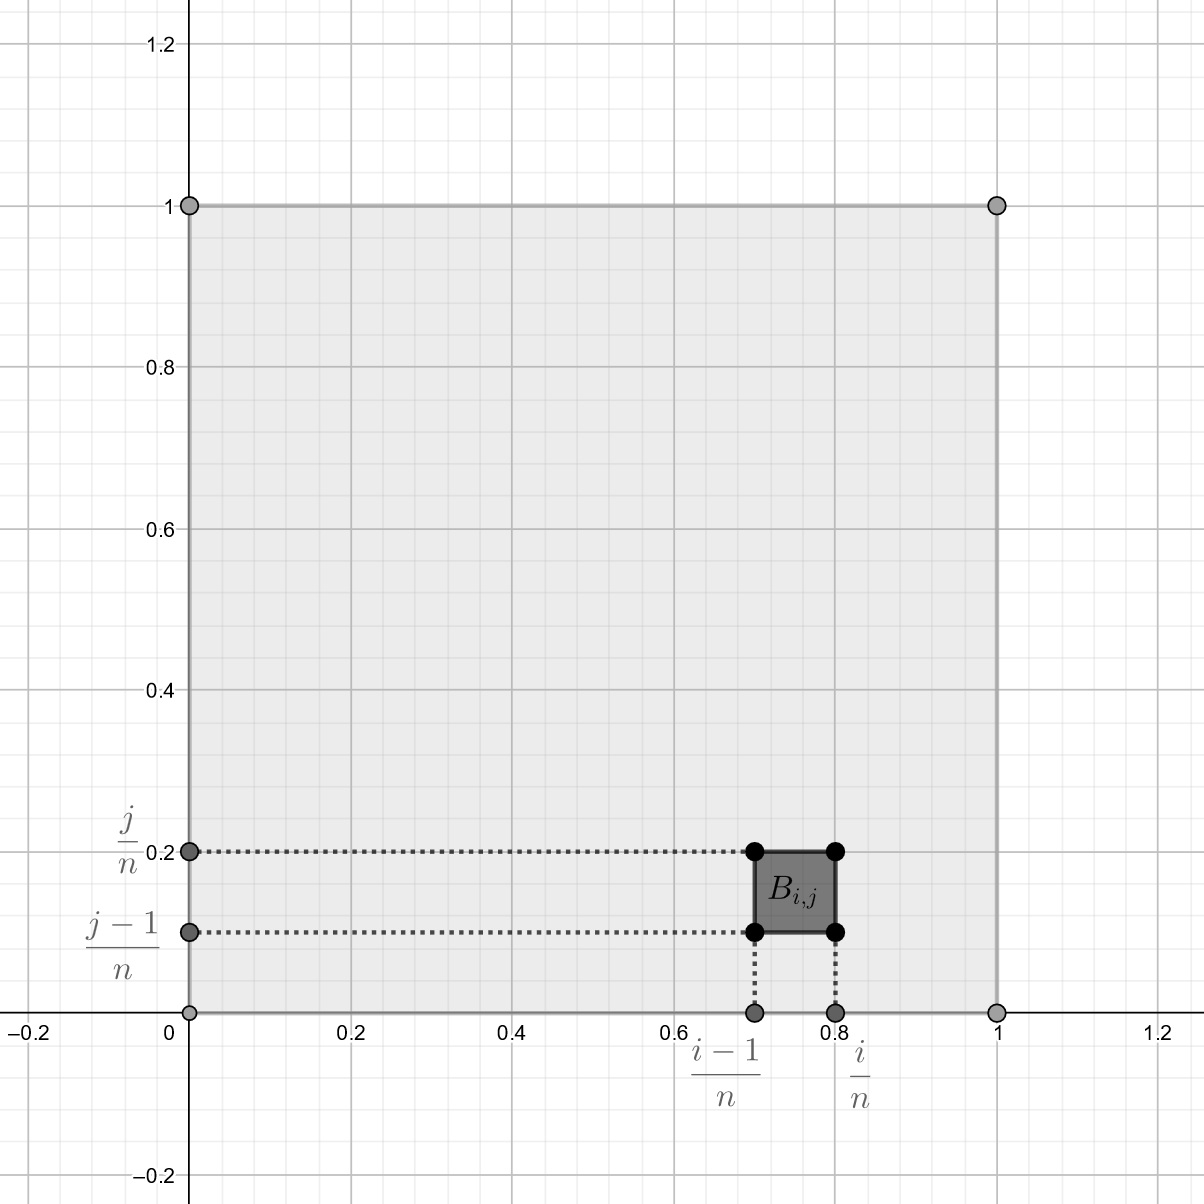
\includegraphics[scale=0.18]{imgs/percolationPlain.png}
			\end{center}
		}
		\only<2>{
			$$\varepsilon_{i,j} \in \left\lbrace 0,1 \right\rbrace \text{ with } \proba{\varepsilon_{i,j} = 1} = p \quad (\text{ i.e. } \varepsilon_{i,j} \sim \mathcal{B}(p) )$$
			$$P = \bigcup_{ \substack{i,j \\ \varepsilon_{i,j}=1} } B_{i,j}$$
			$$Z = \abs{ \left\lbrace (i,j) \mid \epsilon_{i,j}=1 \right\rbrace }$$
			$$D = \frac{Z}{pn^2}$$
			%$$D>0 \iff P \neq \emptyset$$
			%$$\E(D) = 1$$
		}
		\only<3>{
			\begin{center}
				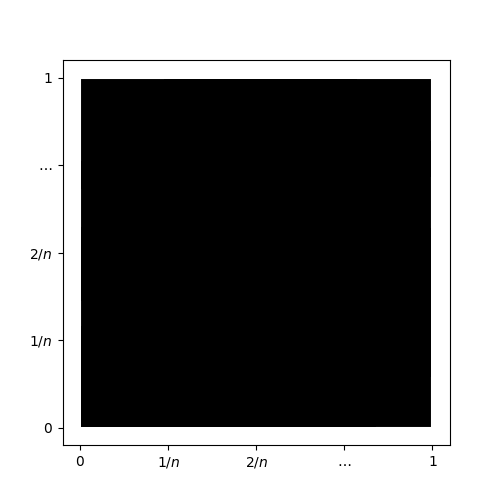
\includegraphics[scale=0.6]{imgs/perc_fig0.png}
			\end{center}
		}
		\only<4>{
			\begin{center}
				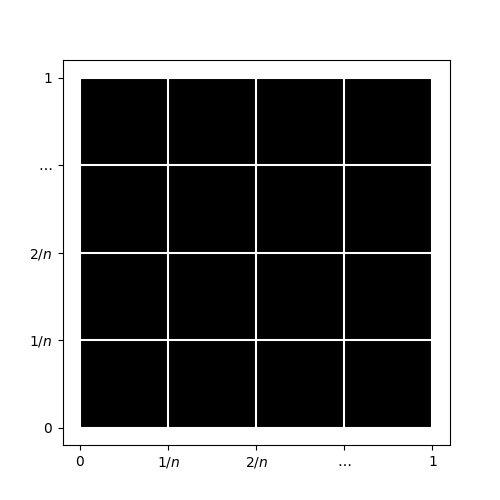
\includegraphics[scale=0.6]{imgs/perc_fig1.png}
			\end{center}
		}
	\end{frame}
	\begin{frame}
		\frametitle{The Percolation Process}
	    \framesubtitle{Recursive: $P_d \sim \rperc{n}{p}{d}$}		
		\only<1-2>{
			$$B_{i,j}^d = \left[\frac{i-1}{n^d},\frac{i}{n^d}\right] \times \left[ \frac{j-1}{n^d},\frac{j}{n^d}\right] $$
		}
		\only<1>{
			\begin{center}
				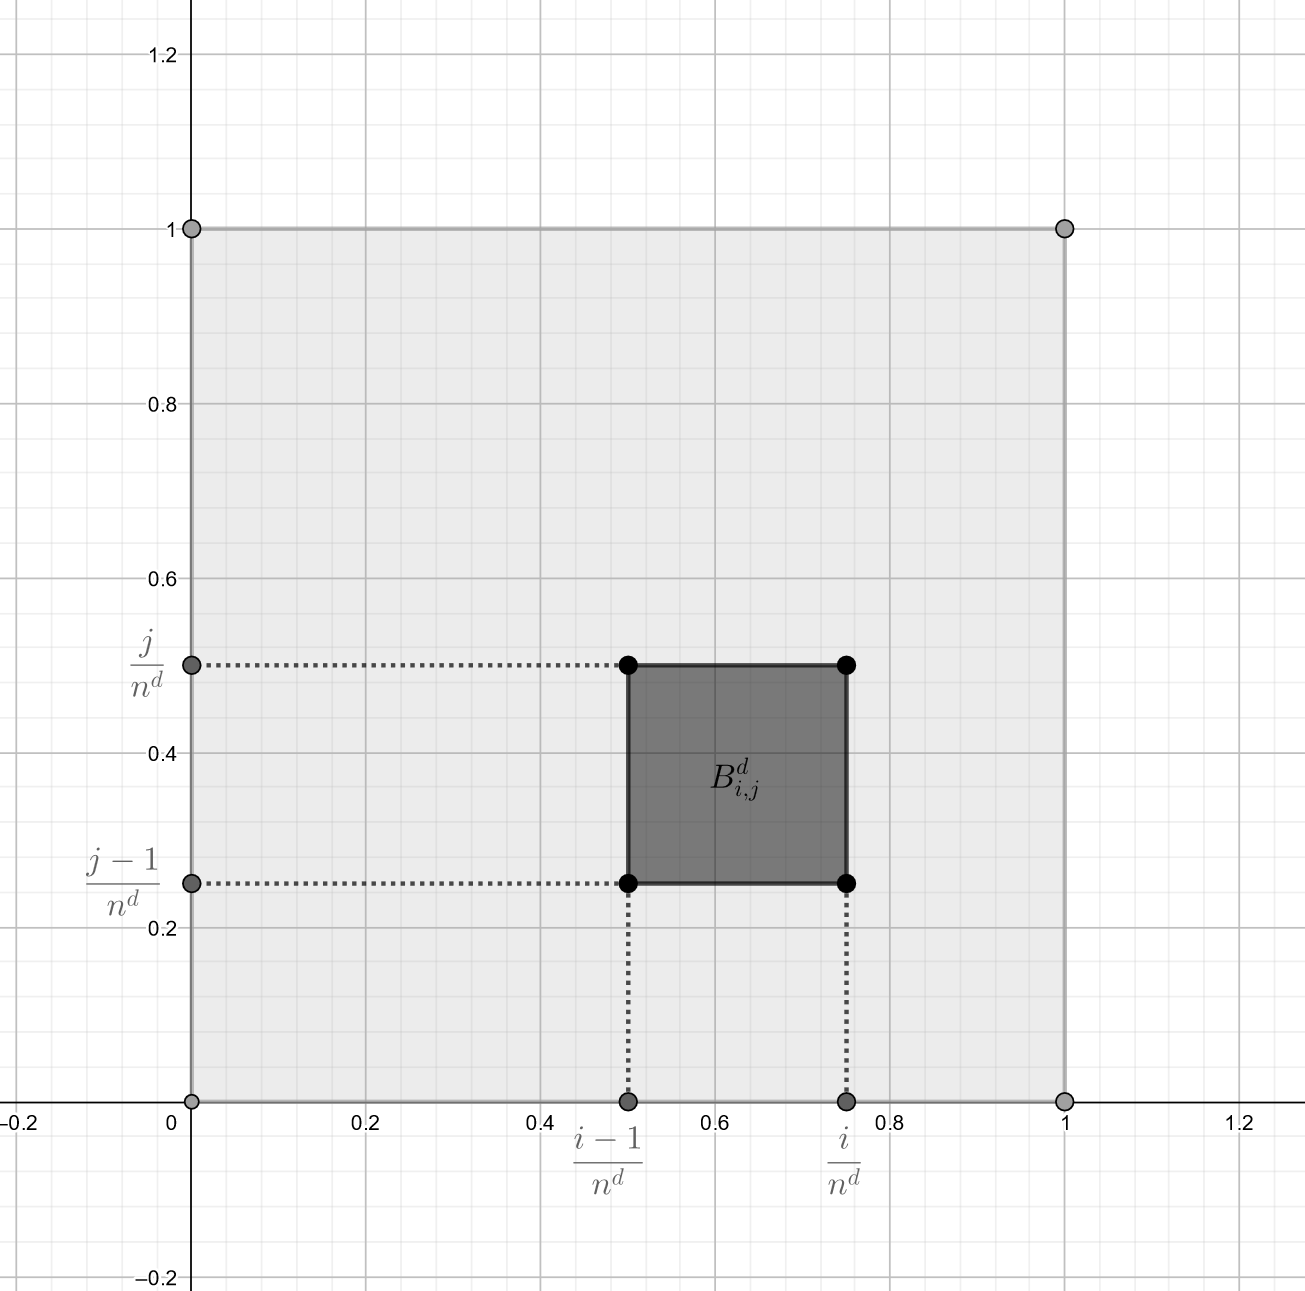
\includegraphics[scale=0.17]{imgs/percolationRecursive.png}
			\end{center}
		}
		\only<2>{
			$$\varepsilon_{i,j}^d \in \left\lbrace 0,1 \right\rbrace \text{ with } \proba{\varepsilon_{i,j}^d = 1} = p \quad (\text{ i.e. } \varepsilon_{i,j}^d \sim \mathcal{B}(p) )$$
			$$P_0 = [0,1]^2
			\quad ; \quad
			P_d = P_{d-1} \bigcap \left( \bigcup_{ \substack{i,j \\
					\varepsilon_{i,j}^d=1} } B_{i,j}^d \right)
			$$
			$$Z_d = \abs{ \left\lbrace  (i,j) \mid \epsilon_{i,j}^d=1 \right\rbrace }$$
			$$D_d = \frac{Z_d}{(pn^2)^d}$$
		}
		\only<3>{
			\begin{center}
				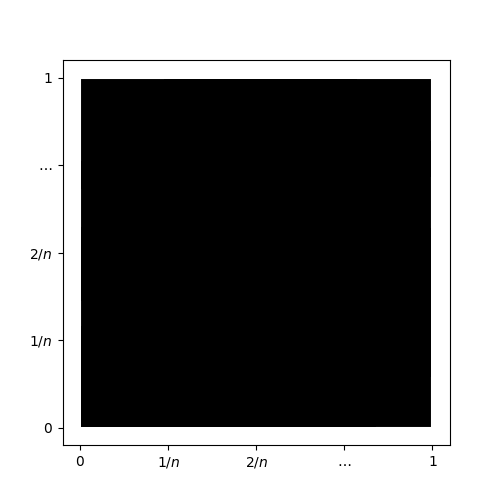
\includegraphics[scale=0.6]{imgs/perc_fig0.png}
			\end{center}
		}
		\only<4>{
			\begin{center}
				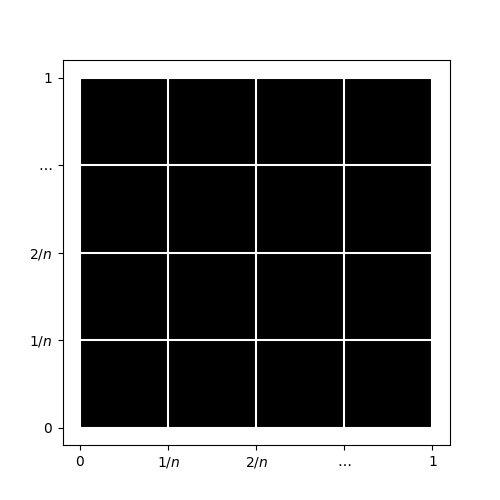
\includegraphics[scale=0.6]{imgs/perc_fig1.png}
			\end{center}
		}
		\only<5>{
			\begin{center}
				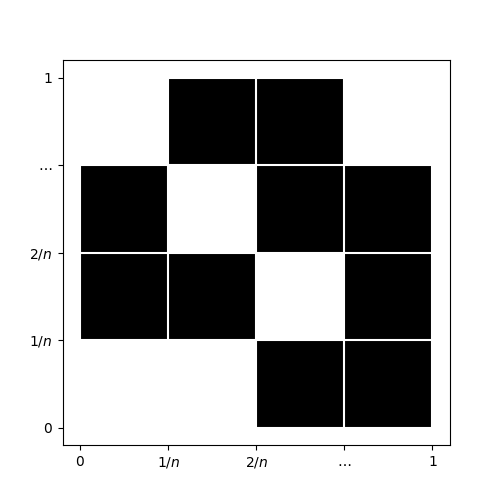
\includegraphics[scale=0.6]{imgs/perc_fig2.png}
			\end{center}
		}
	\end{frame}
	\begin{frame}
		\frametitle{The Percolation Process}
		\framesubtitle{Limit: $P_{\infty} \sim \perc{n}{p}$}		
		$$P_{\infty} = \bigcap_{d \in \N} P_d$$
		$$D_{\infty} = \lim_{d \to \infty} D_d$$
		\vspace*{1cm}
		\pause
		$$D_{\infty}>0 \iff P_{\infty} \neq \emptyset$$
		$$\E(D_{\infty}) = 1$$
	\end{frame}

	\begin{frame}
	    \frametitle{The Percolation Process}
		\framesubtitle{Example for $n=2$}
		\begin{center}
			\only<1>{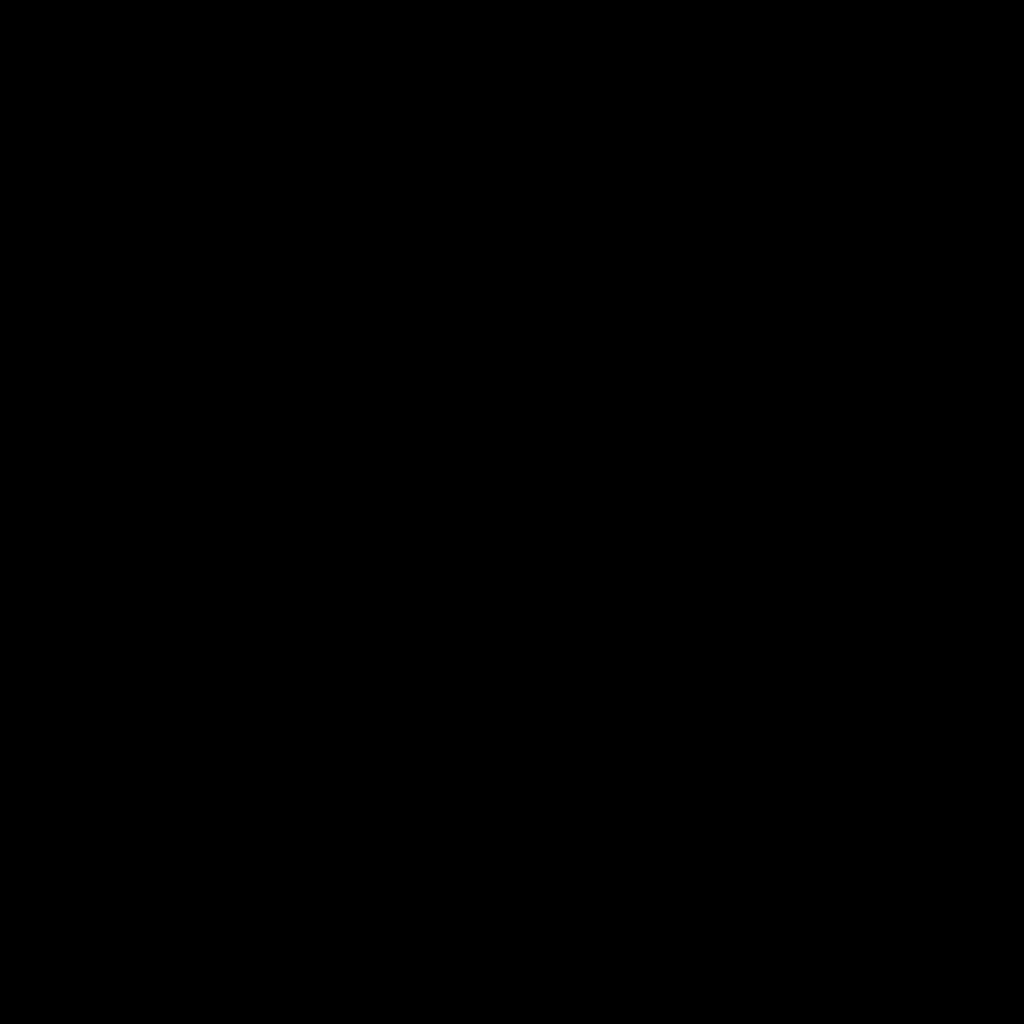
\includegraphics[scale=1.25]{imgs/perc2step0.png}}
			\only<2>{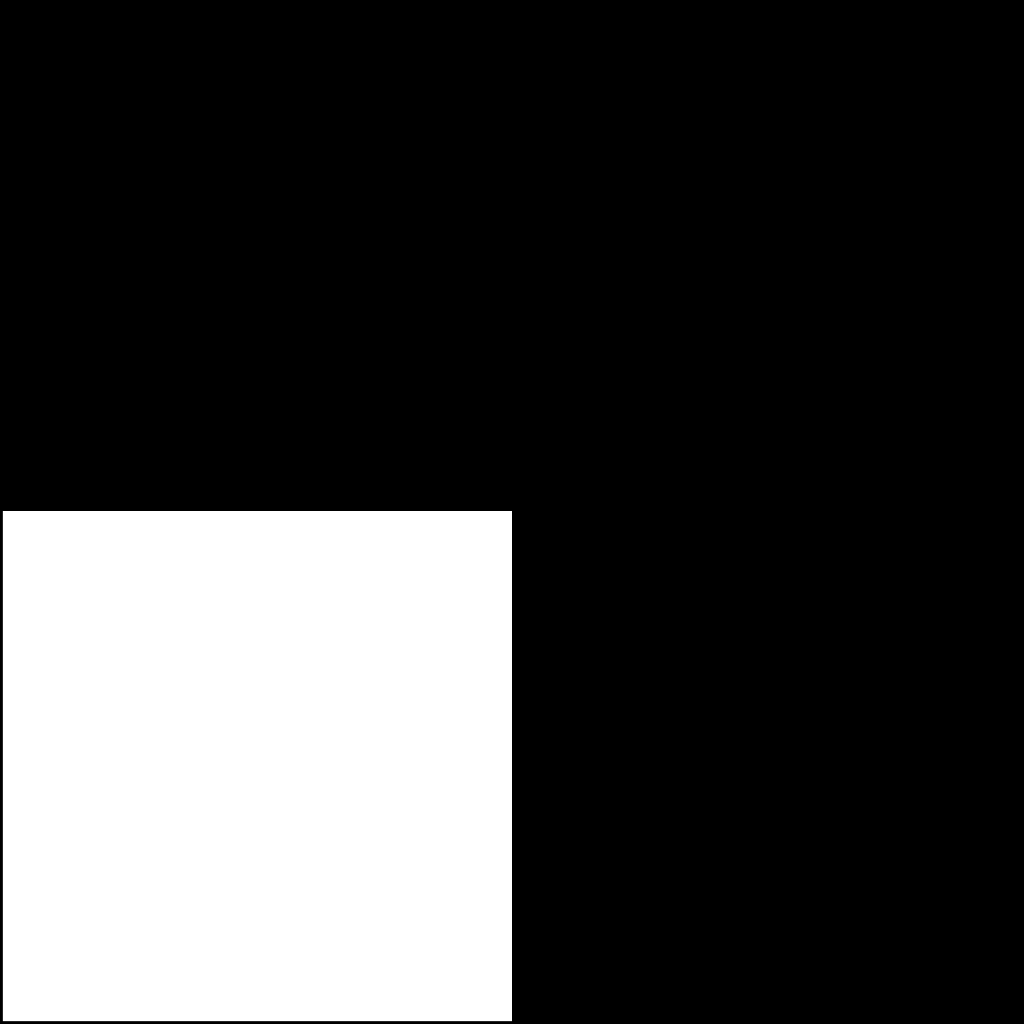
\includegraphics[scale=1.25]{imgs/perc2step1.png}}
			\only<3>{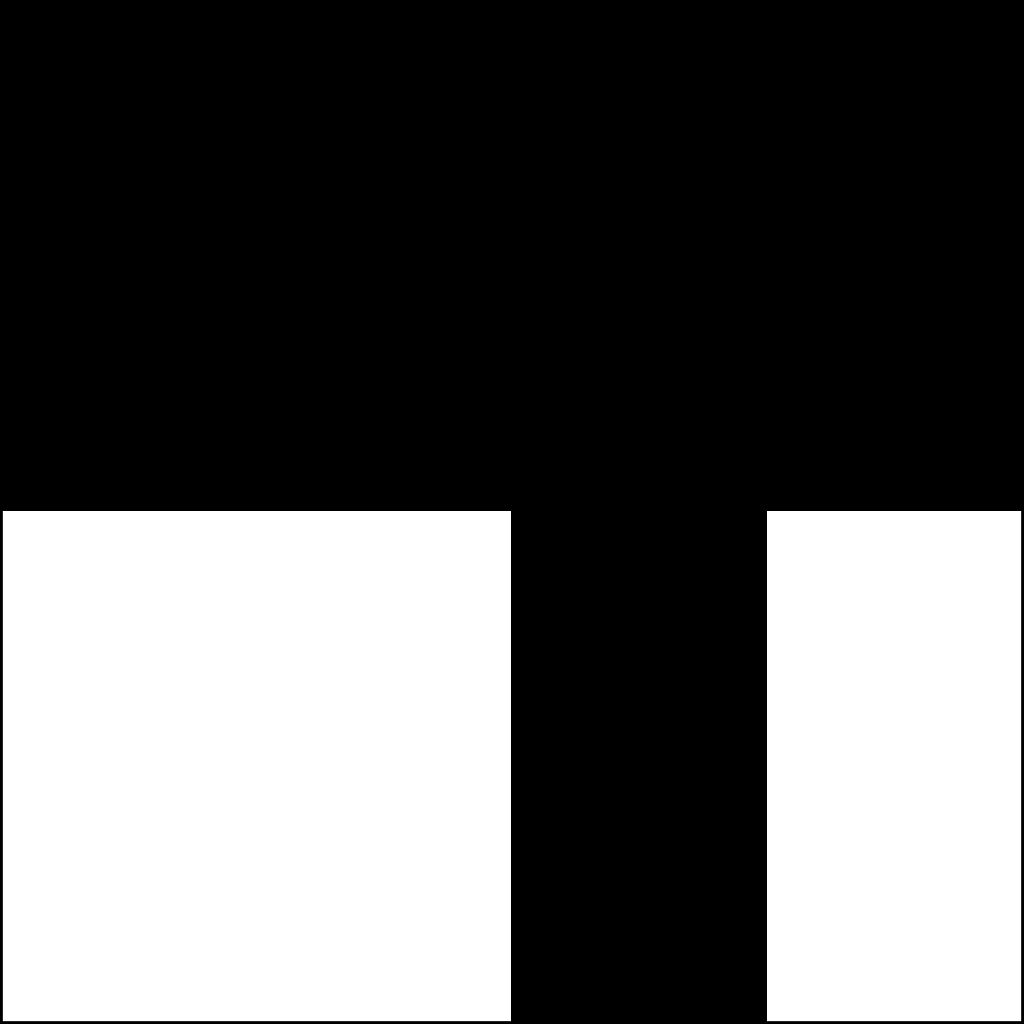
\includegraphics[scale=1.25]{imgs/perc2step2.png}}
			\only<4>{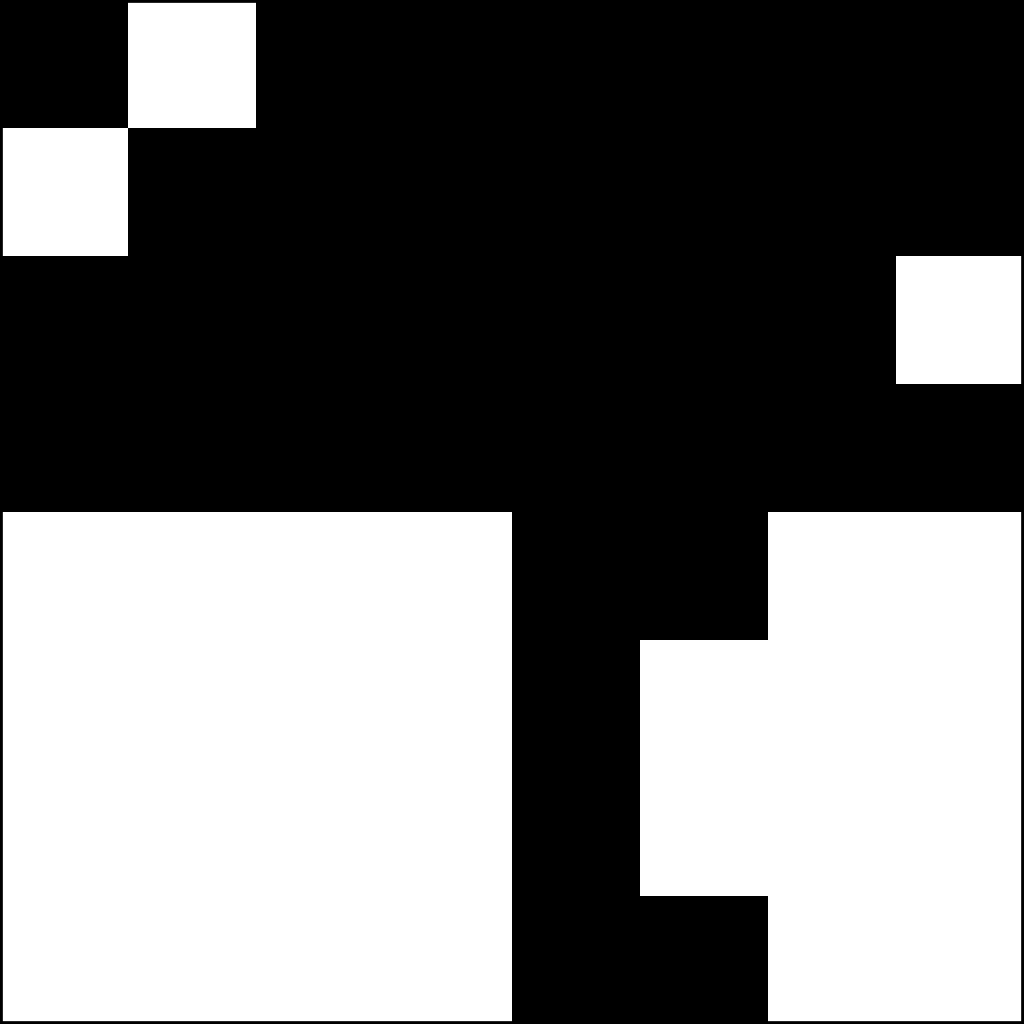
\includegraphics[scale=1.25]{imgs/perc2step3.png}}
			\only<5>{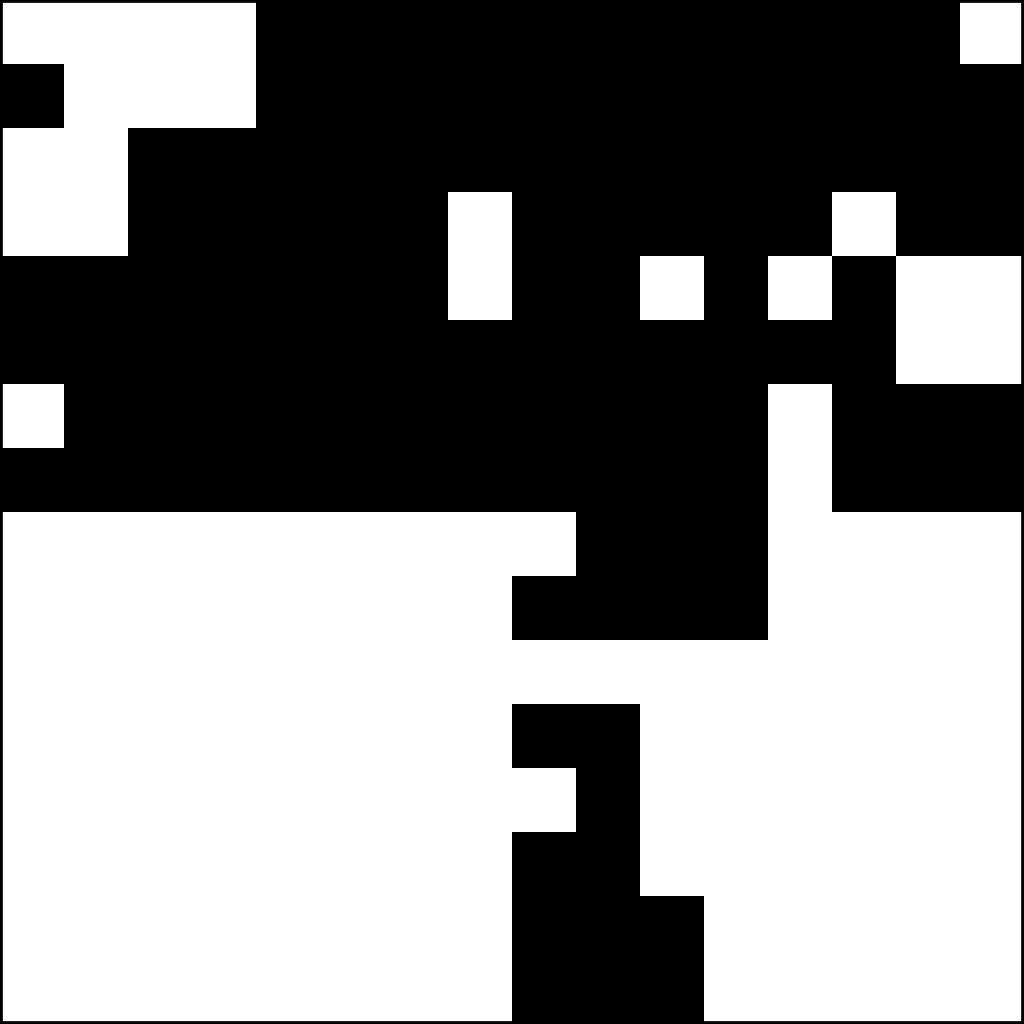
\includegraphics[scale=1.25]{imgs/perc2step4.png}}
			\only<6>{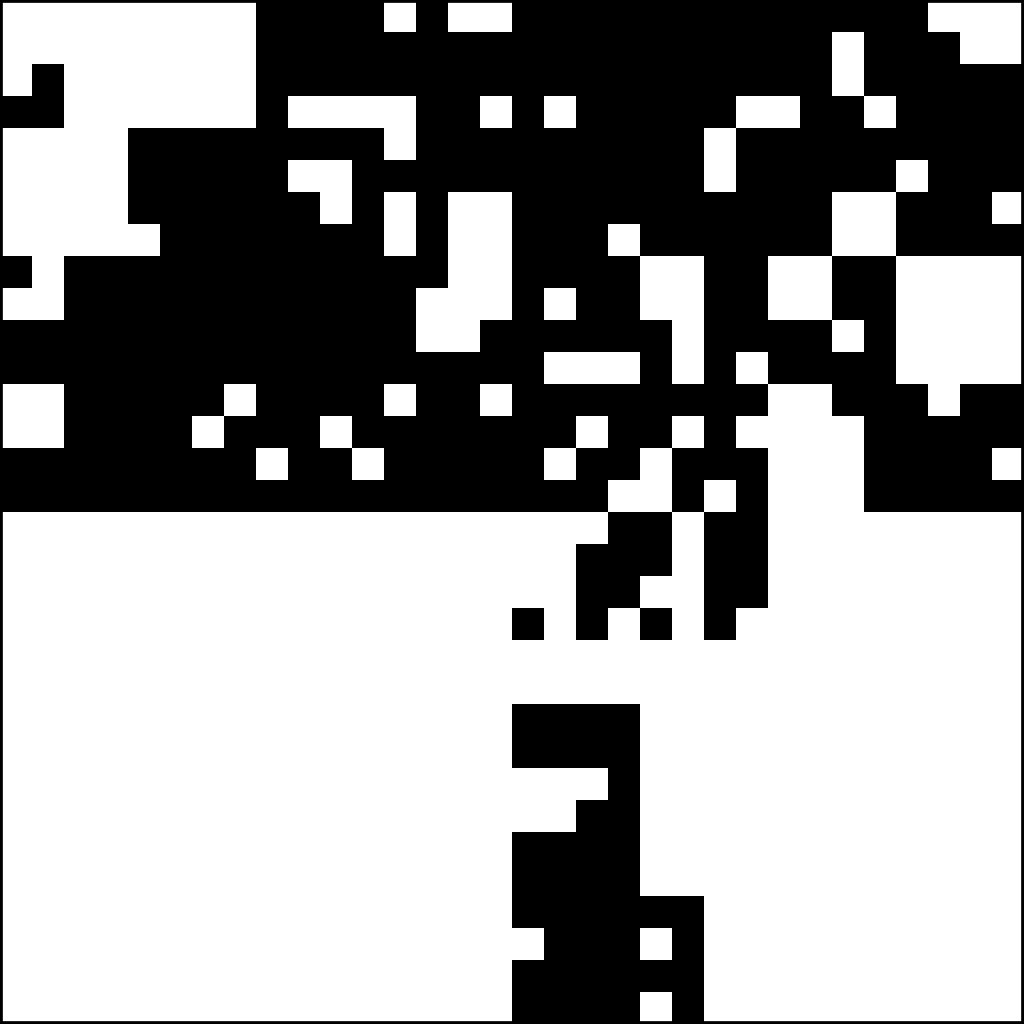
\includegraphics[scale=1.25]{imgs/perc2step5.png}}
			\only<7>{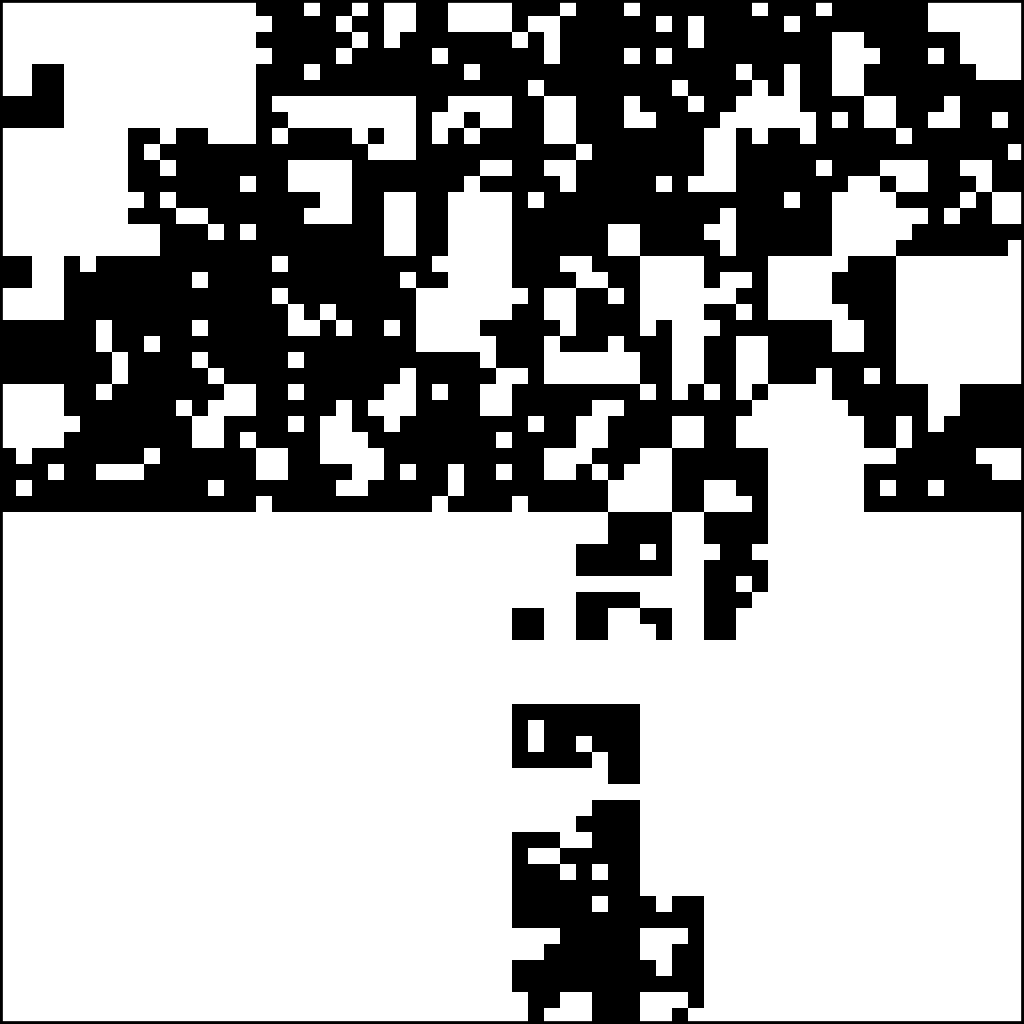
\includegraphics[scale=1.25]{imgs/perc2step6.png}}
			\only<8>{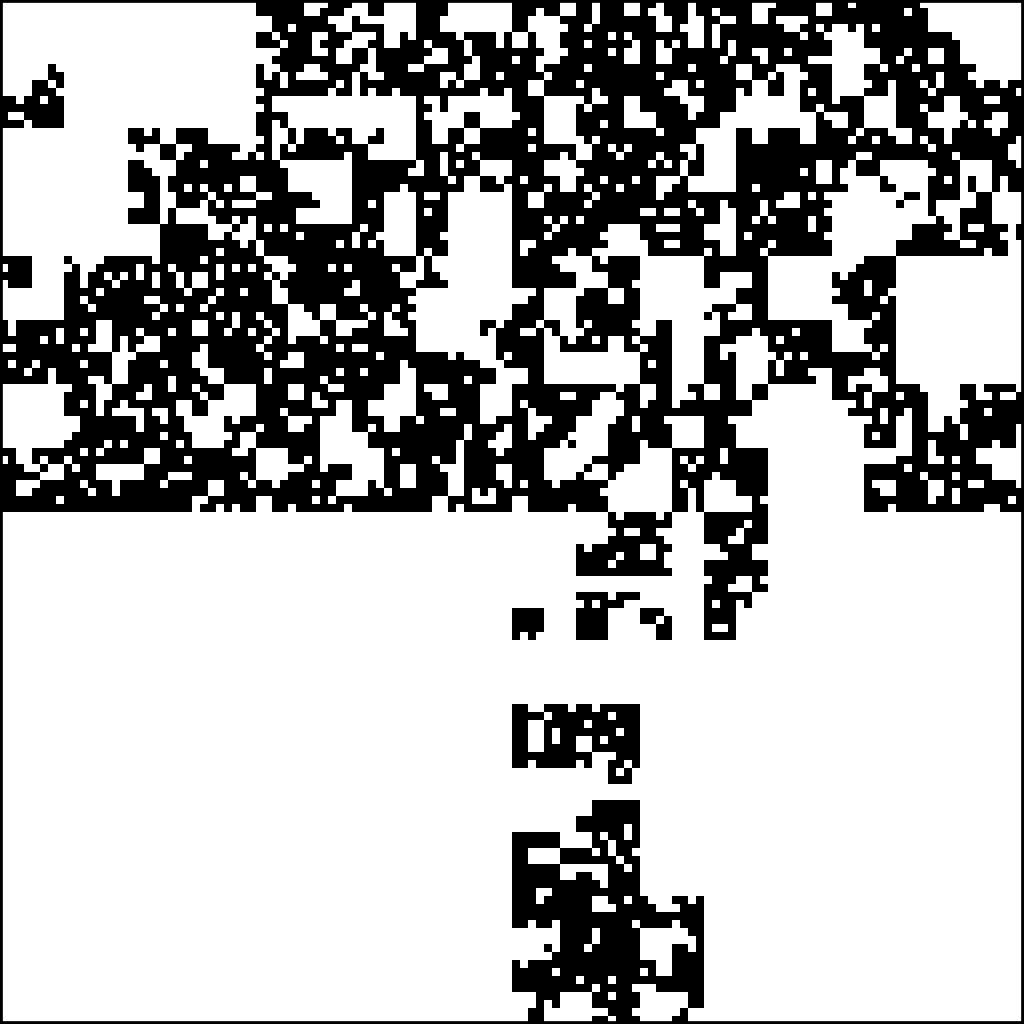
\includegraphics[scale=1.25]{imgs/perc2step7.png}}
			\only<9>{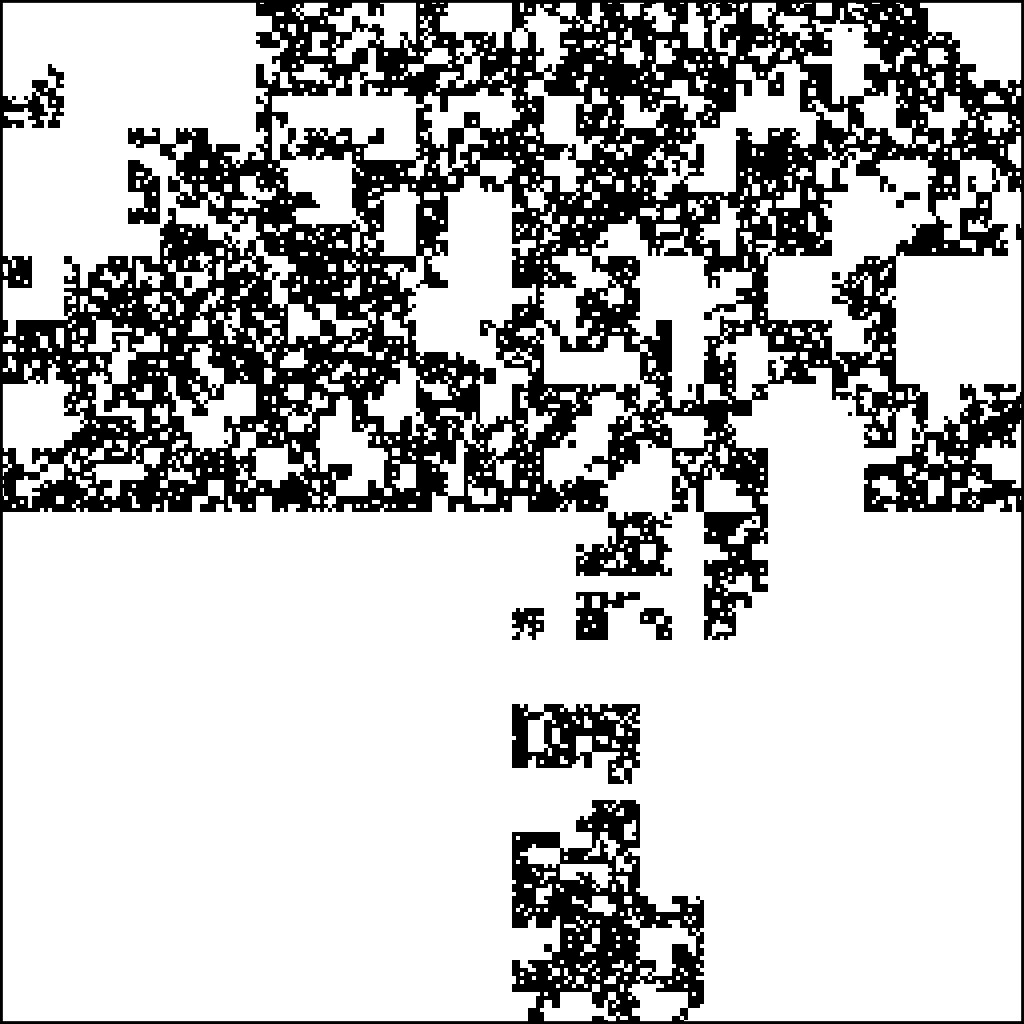
\includegraphics[scale=1.25]{imgs/perc2step8.png}}
			\only<10>{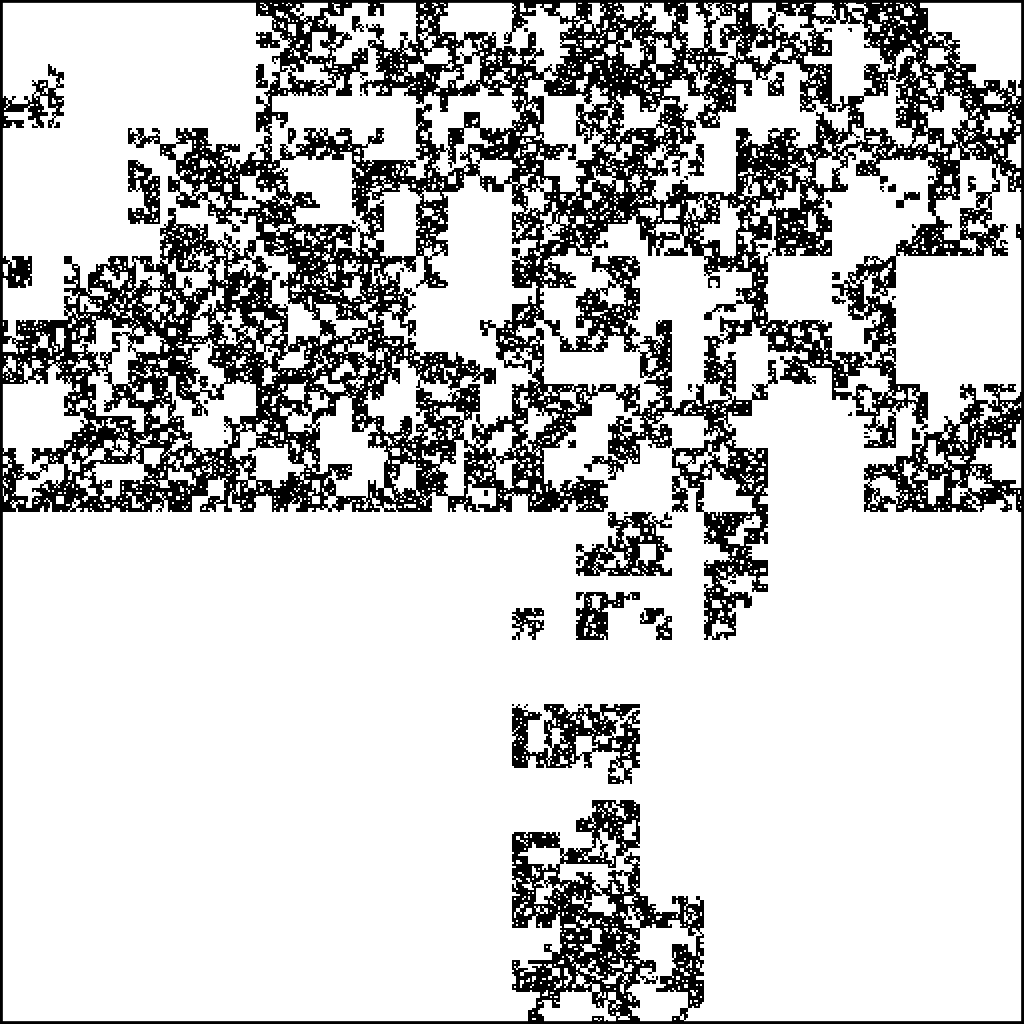
\includegraphics[scale=1.25]{imgs/perc2step9.png}}
		\end{center}
	\end{frame}
	\begin{frame}
	    \frametitle{The Percolation Process}
		\framesubtitle{Example for $n=3$}
		\begin{center}
			\only<1>{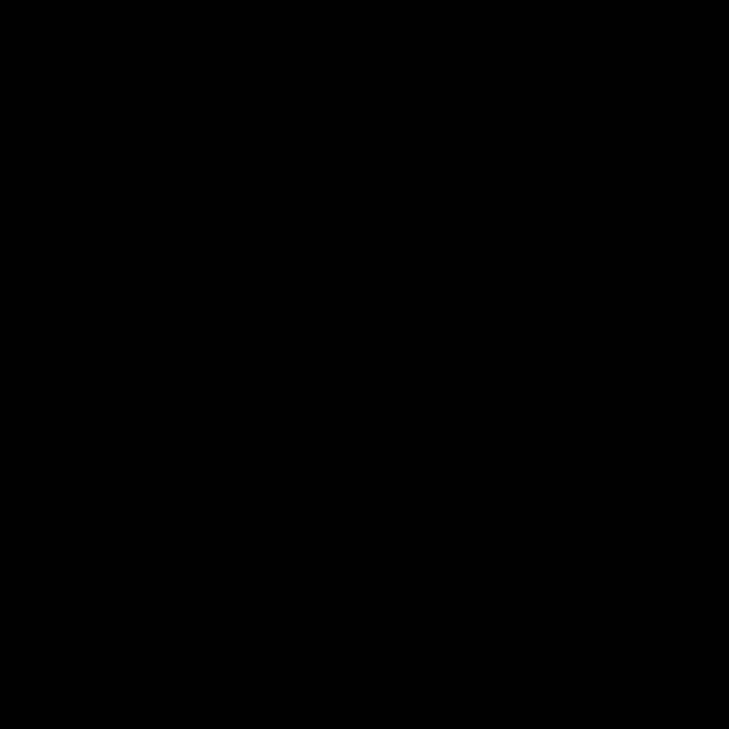
\includegraphics[scale=0.85]{imgs/perc3step0.png}}
			\only<2>{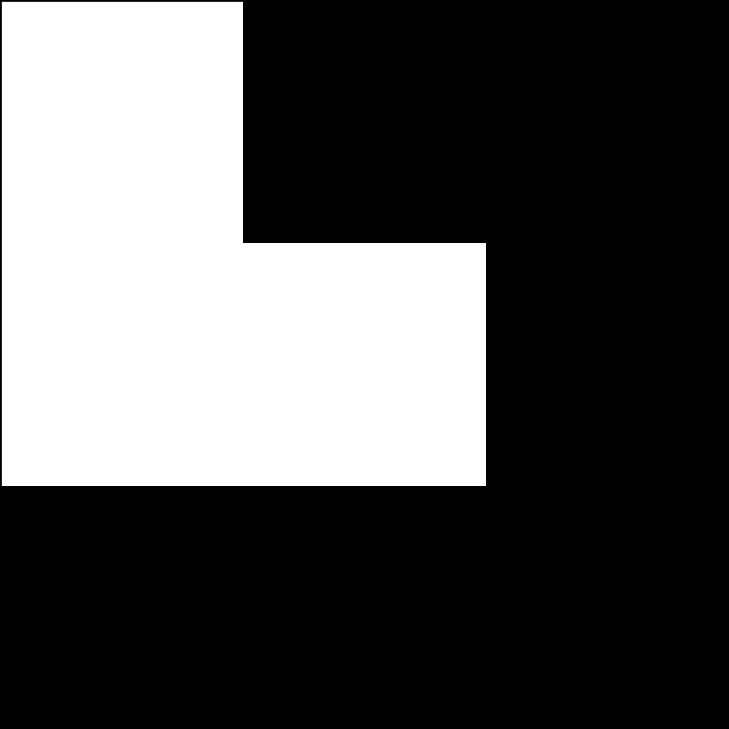
\includegraphics[scale=0.85]{imgs/perc3step1.png}}
			\only<3>{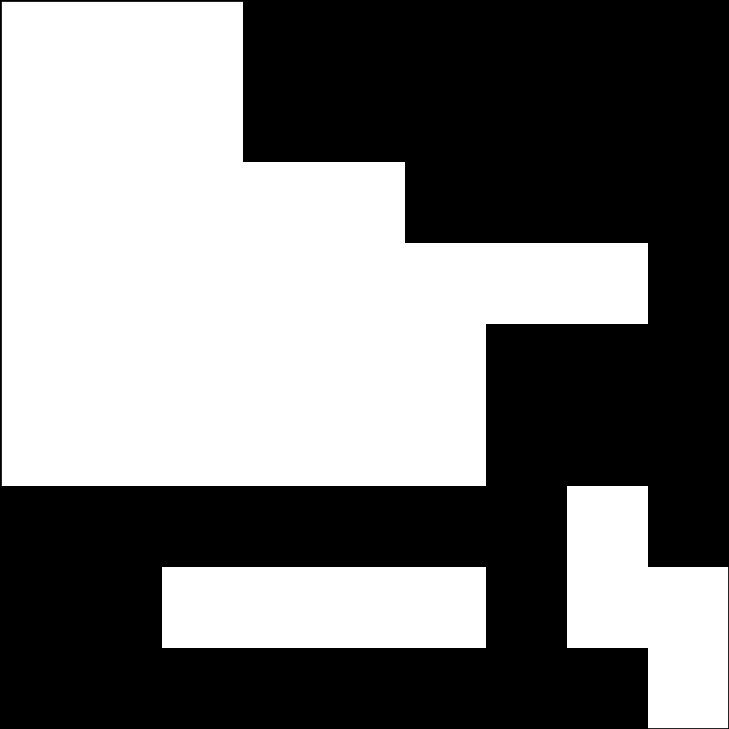
\includegraphics[scale=0.85]{imgs/perc3step2.png}}
			\only<4>{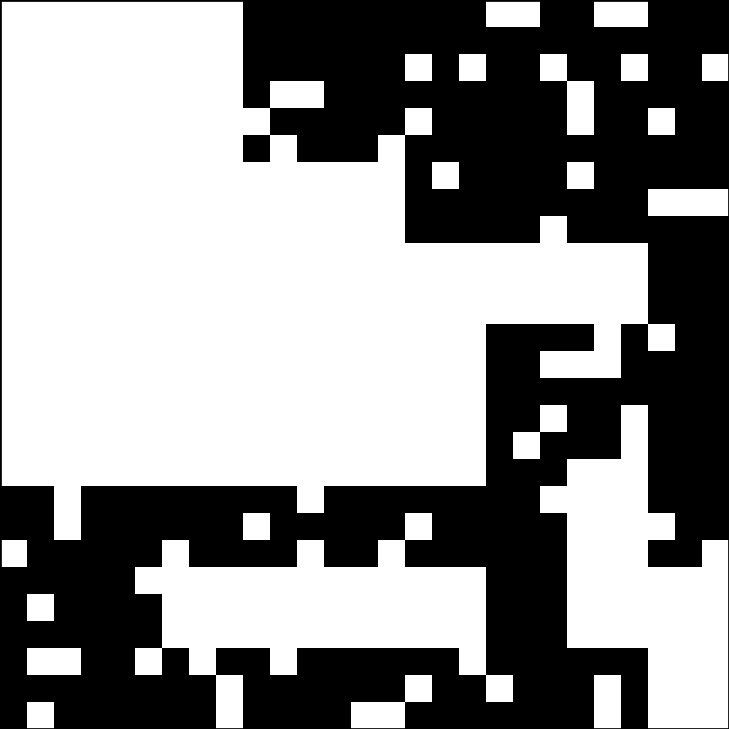
\includegraphics[scale=0.85]{imgs/perc3step3.png}}
			\only<5>{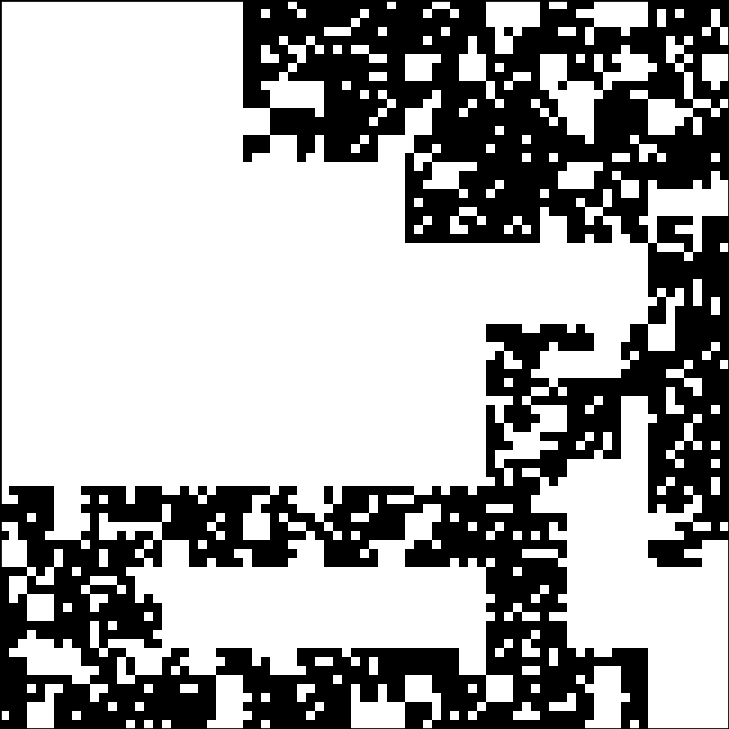
\includegraphics[scale=0.85]{imgs/perc3step4.png}}
			\only<6>{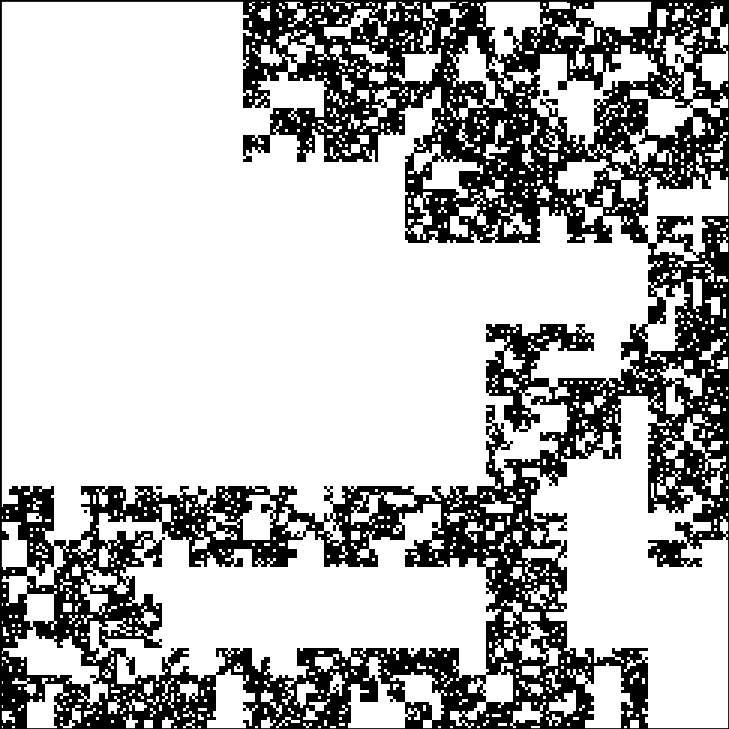
\includegraphics[scale=0.85]{imgs/perc3step5.png}}
		\end{center}
	\end{frame}
	\begin{frame}
		\frametitle{The Percolation Process}
		\framesubtitle{Example for $n=5$}
		\begin{center}
			\only<1>{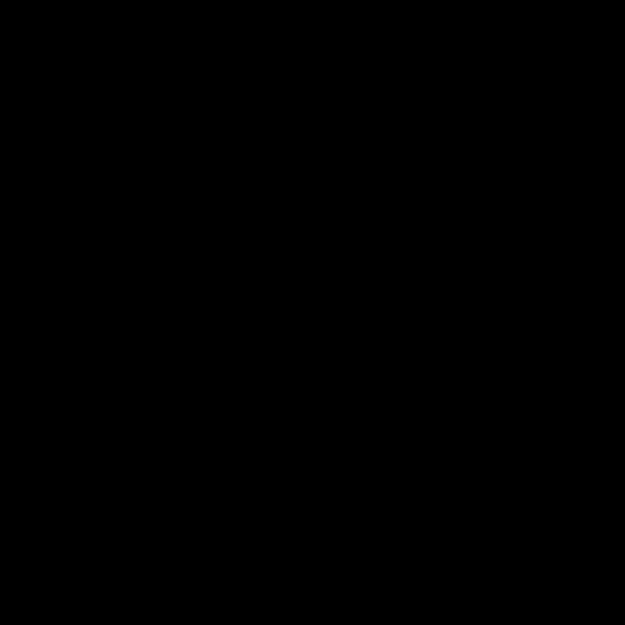
\includegraphics[scale=0.5]{imgs/perc5step0.png}}
			\only<2>{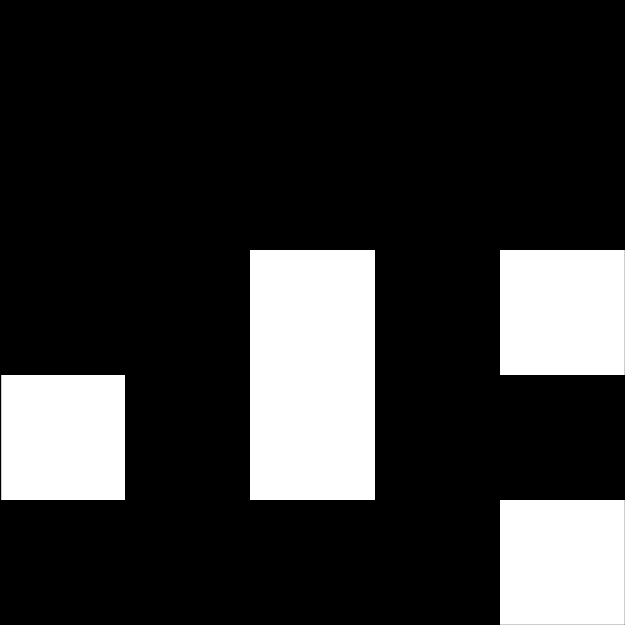
\includegraphics[scale=0.5]{imgs/perc5step1.png}}
			\only<3>{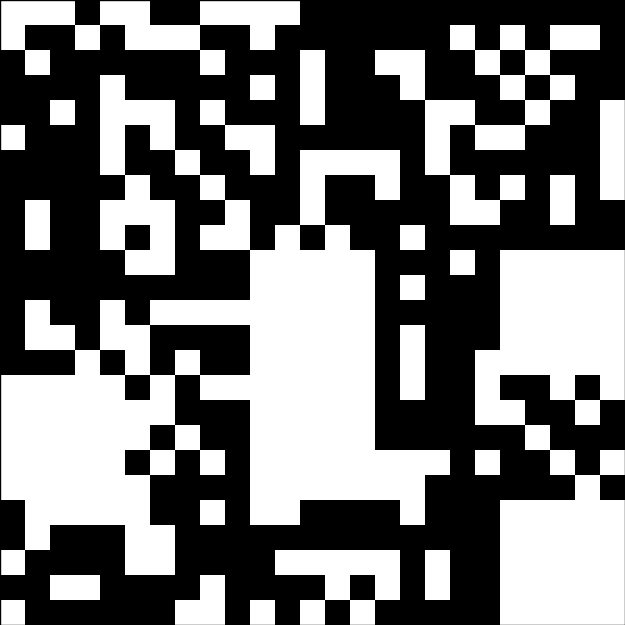
\includegraphics[scale=0.5]{imgs/perc5step2.png}}
			\only<4>{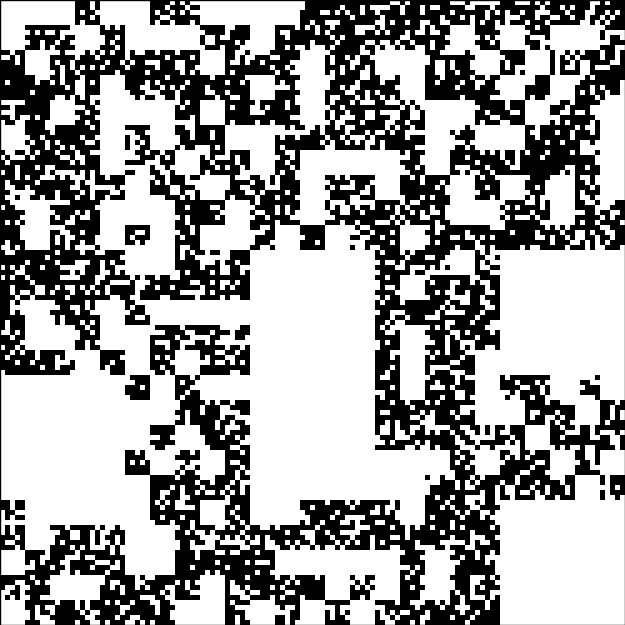
\includegraphics[scale=0.5]{imgs/perc5step3.png}}
		\end{center}
	\end{frame}

	\begin{frame}
		\frametitle{Dimensions}
		\framesubtitle{Intuition}
		\begin{itemize}
			\pause
			\item[$1D$:] Scale by $\lambda$ $\iff$ Lengths multiplied by $\lambda^1$
			\pause
			\item[$2D$:] Scale by $\lambda$ $\iff$ Areas multiplied by $\lambda^2$
			\pause
			\item[$3D$:] Scale by $\lambda$ $\iff$ Volumes multiplied by $\lambda^3$
			\pause
			\item[$\dots$]
			\item[$nD$:] Scale by $\lambda$ $\iff$ n-Dim. Volumes multiplies by $\lambda^n \quad \forall n \in \N$
			\pause
			\item[\color{purple} $\dots$]
			\item[\color{red} $\alpha D$:] \color{brickred} Scale by $\lambda$ $\iff$ n-Dim. Volumes multiplies by $\lambda^{\alpha} \quad \forall \alpha \in \R^+$
		\end{itemize}
	\end{frame}
	\begin{frame}
		\frametitle{Dimensions}
		\framesubtitle{Percolation dimensions}
		For $P \sim \perc{n}{p}$, scaling by $n$ gives $pn^2$ copies of $P$.
		\begin{center}
			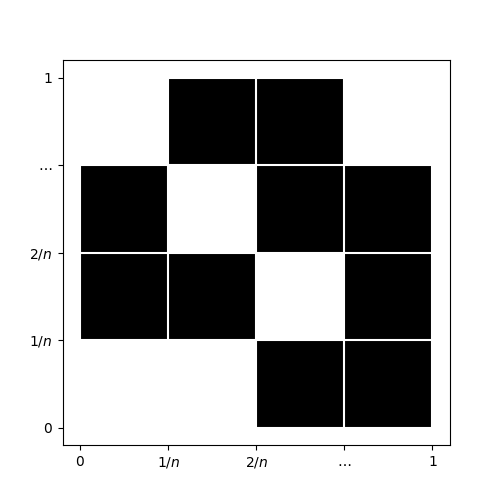
\includegraphics[scale=0.4]{imgs/perc_fig2.png}
		\end{center}
		So $\dim(P) = pn^2$.
		
	\end{frame}
	
	\begin{frame}
	    \frametitle{Types of Crossings}
		\begin{center}
			\only<1>{
				\framesubtitle{Straight}
				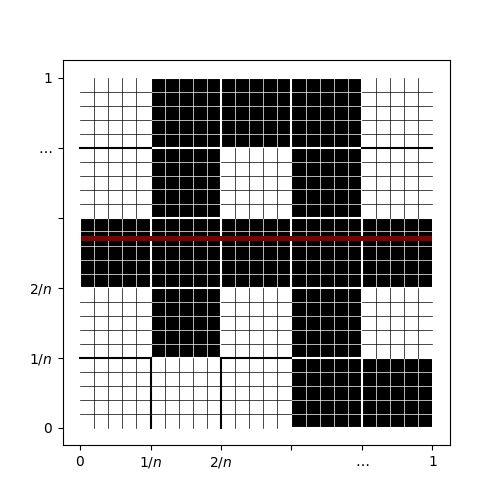
\includegraphics[scale=0.6]{imgs/crossing_fig_straight.png}
			}
			\only<2>{
				\framesubtitle{Semi-Straight}
				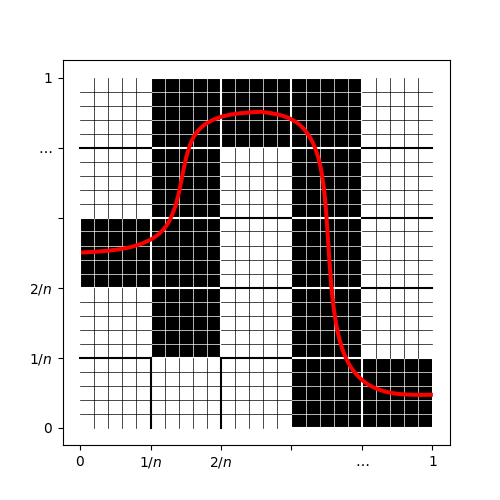
\includegraphics[scale=0.6]{imgs/crossing_fig_semi_straight.png}
			}
			\only<3>{
				\framesubtitle{Non-Straight}
				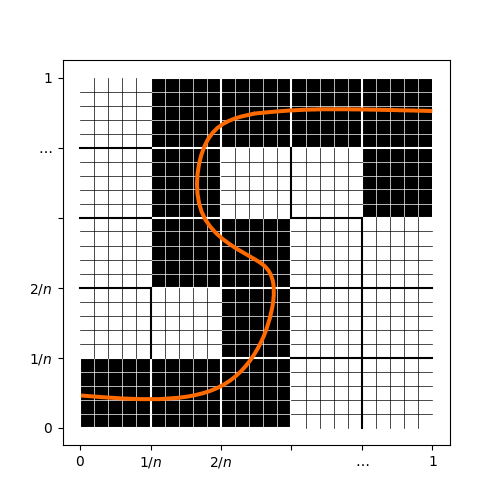
\includegraphics[scale=0.6]{imgs/crossing_fig.png}
			}
		\end{center}
	\end{frame}

	\begin{frame}
		\frametitle{Finding Crossings}
		\framesubtitle{Example for $n=2$}
		\begin{center}
			\only<1>{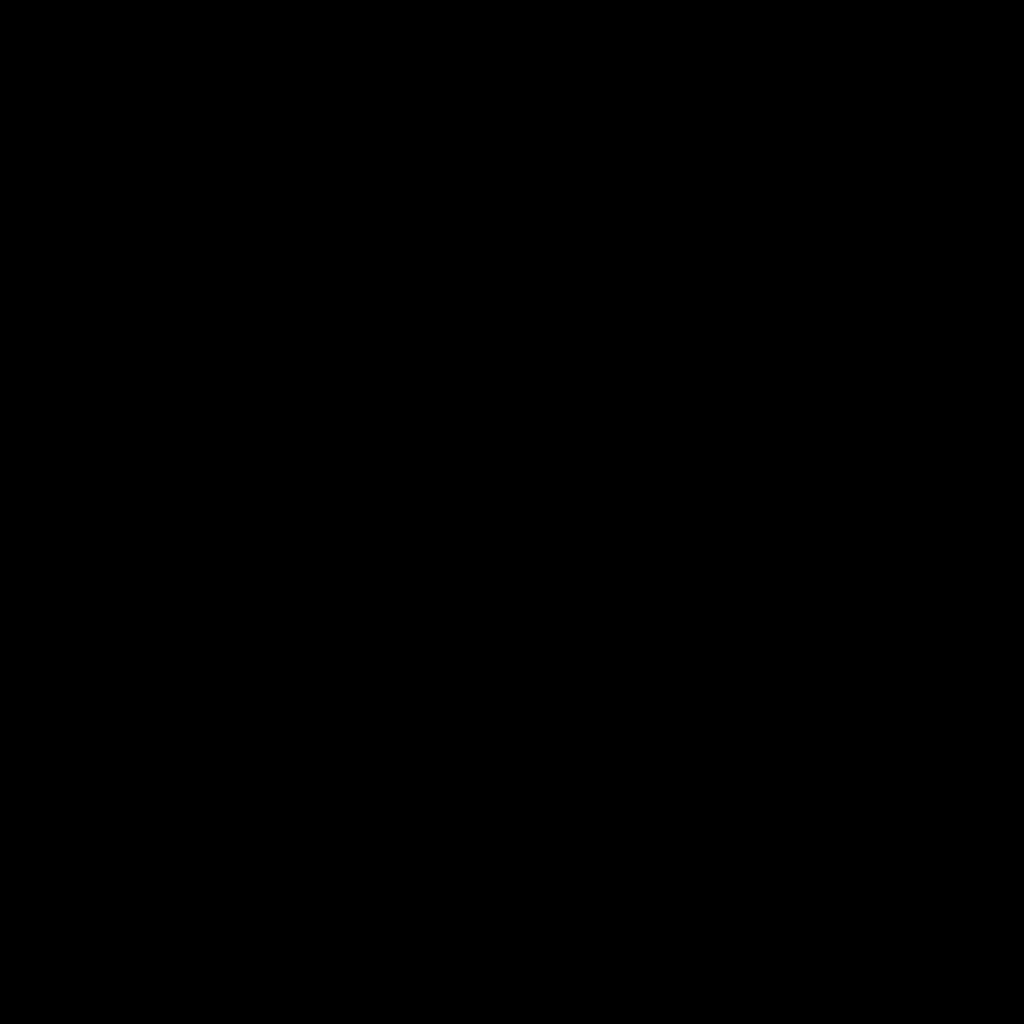
\includegraphics[scale=1.25]{imgs/perc2step0.png}}
			\only<2>{
\includegraphics[scale=1.25]{imgs/perc2step0_crossing.png}}
			\only<3>{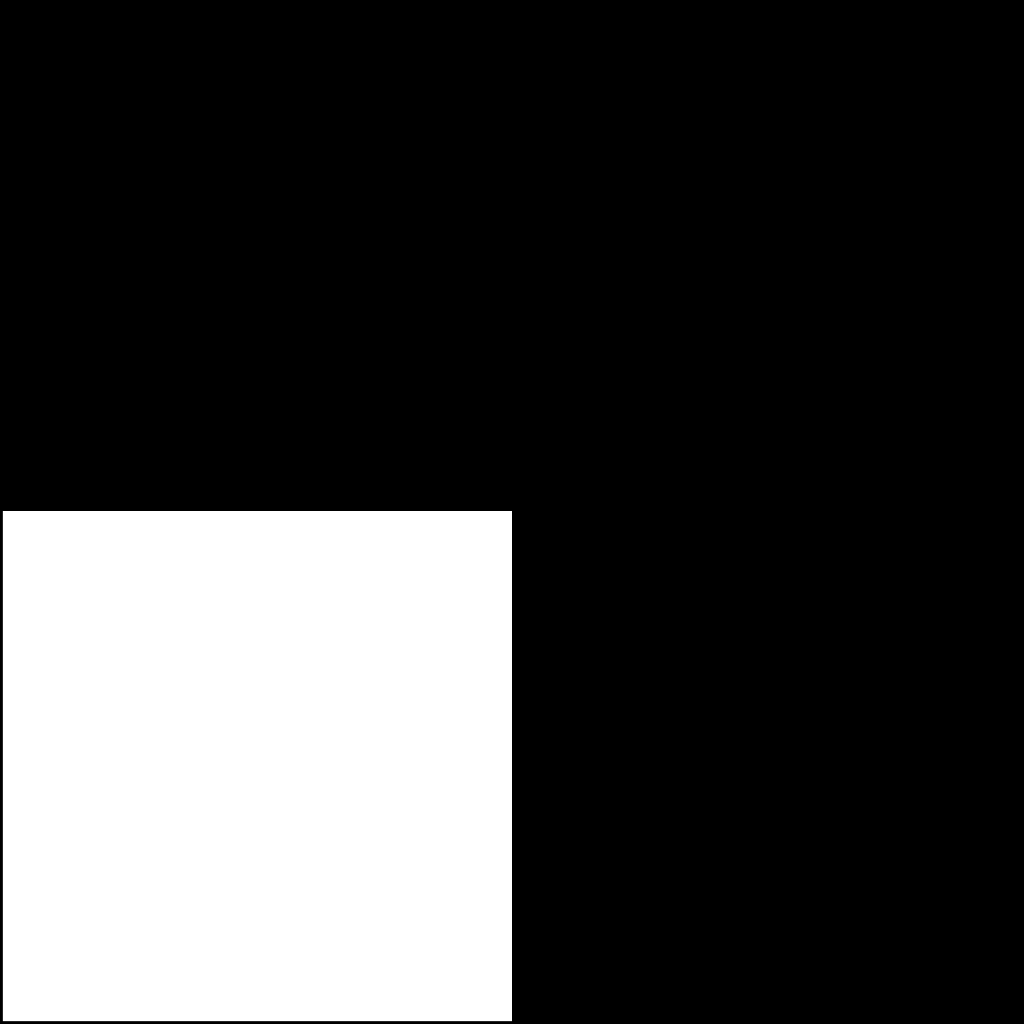
\includegraphics[scale=1.25]{imgs/perc2step1.png}}
			\only<4>{
\includegraphics[scale=1.25]{imgs/perc2step1_crossing.png}}
			\only<5>{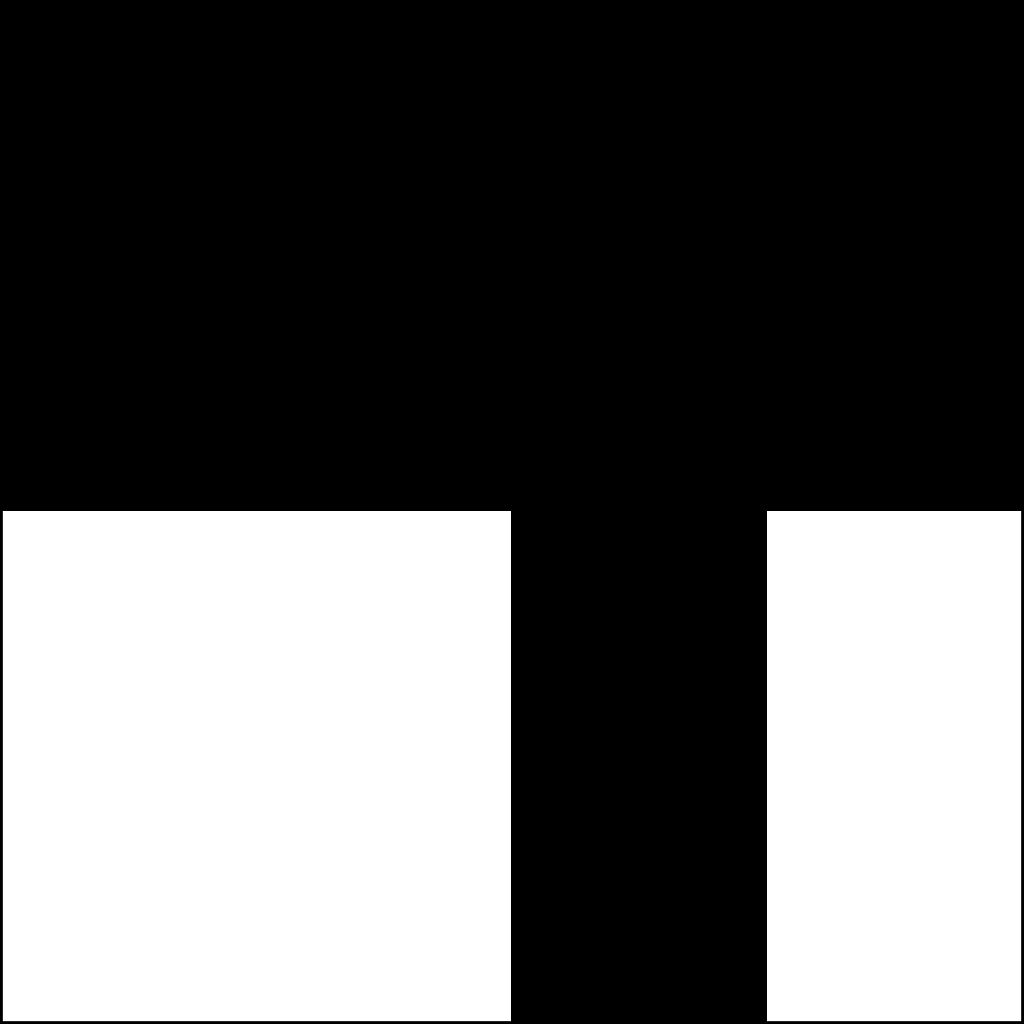
\includegraphics[scale=1.25]{imgs/perc2step2.png}}
			\only<6>{
\includegraphics[scale=1.25]{imgs/perc2step2_crossing.png}}
			\only<7>{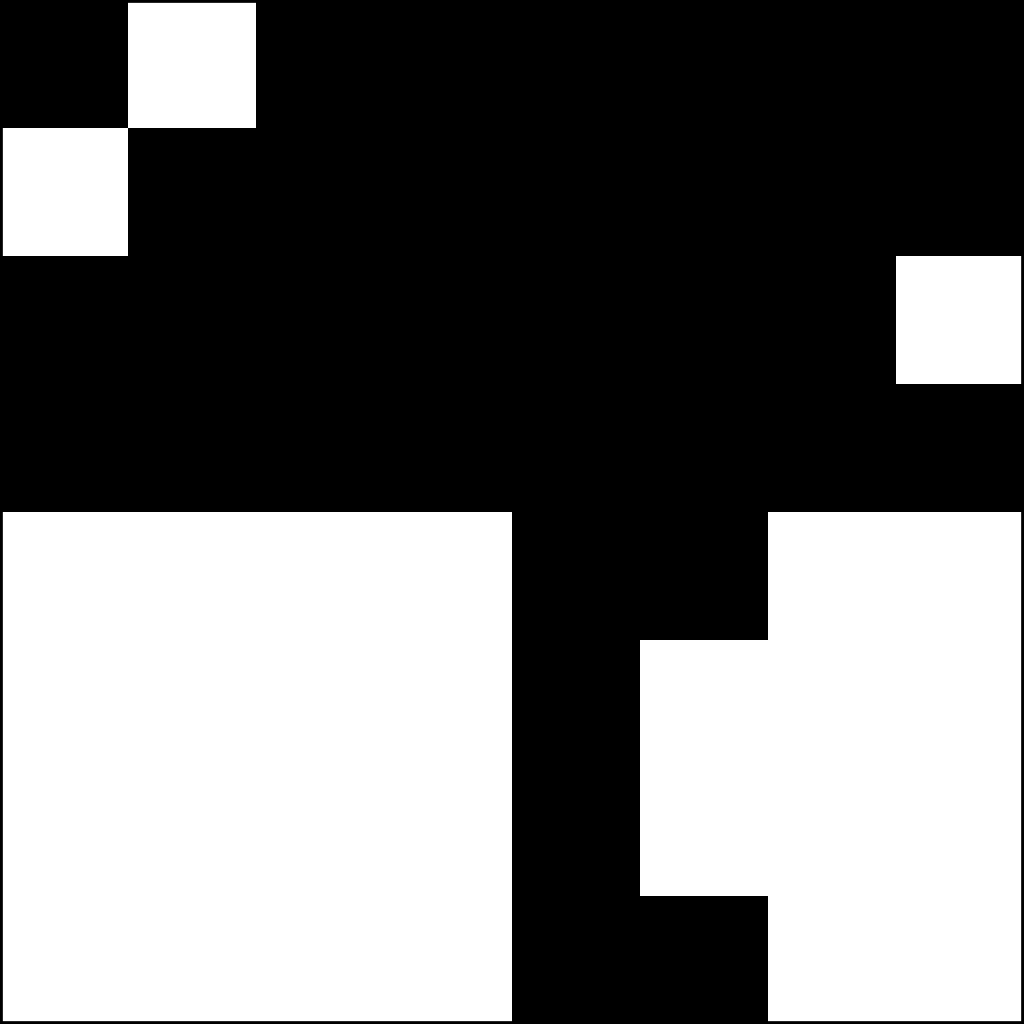
\includegraphics[scale=1.25]{imgs/perc2step3.png}}
			\only<8>{
\includegraphics[scale=1.25]{imgs/perc2step3_crossing.png}}
			\only<9>{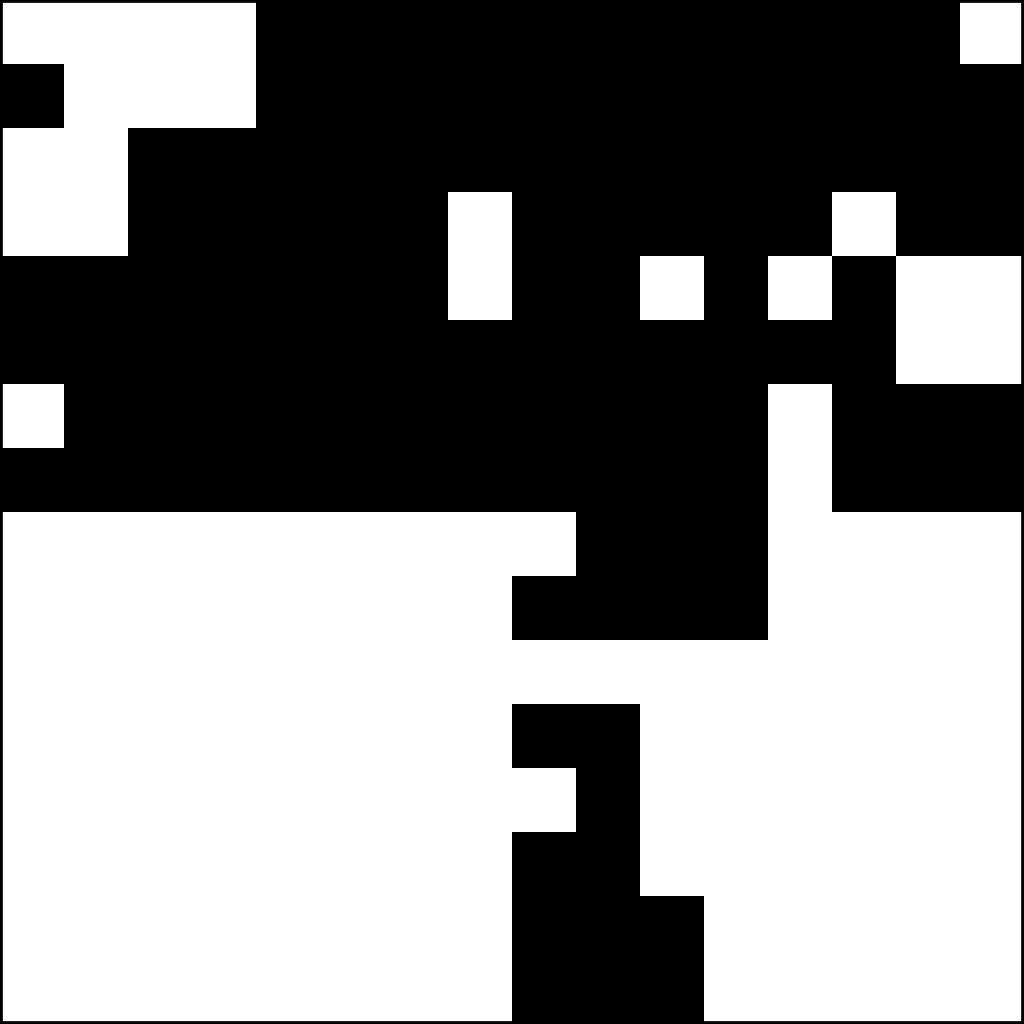
\includegraphics[scale=1.25]{imgs/perc2step4.png}}
			\only<10>{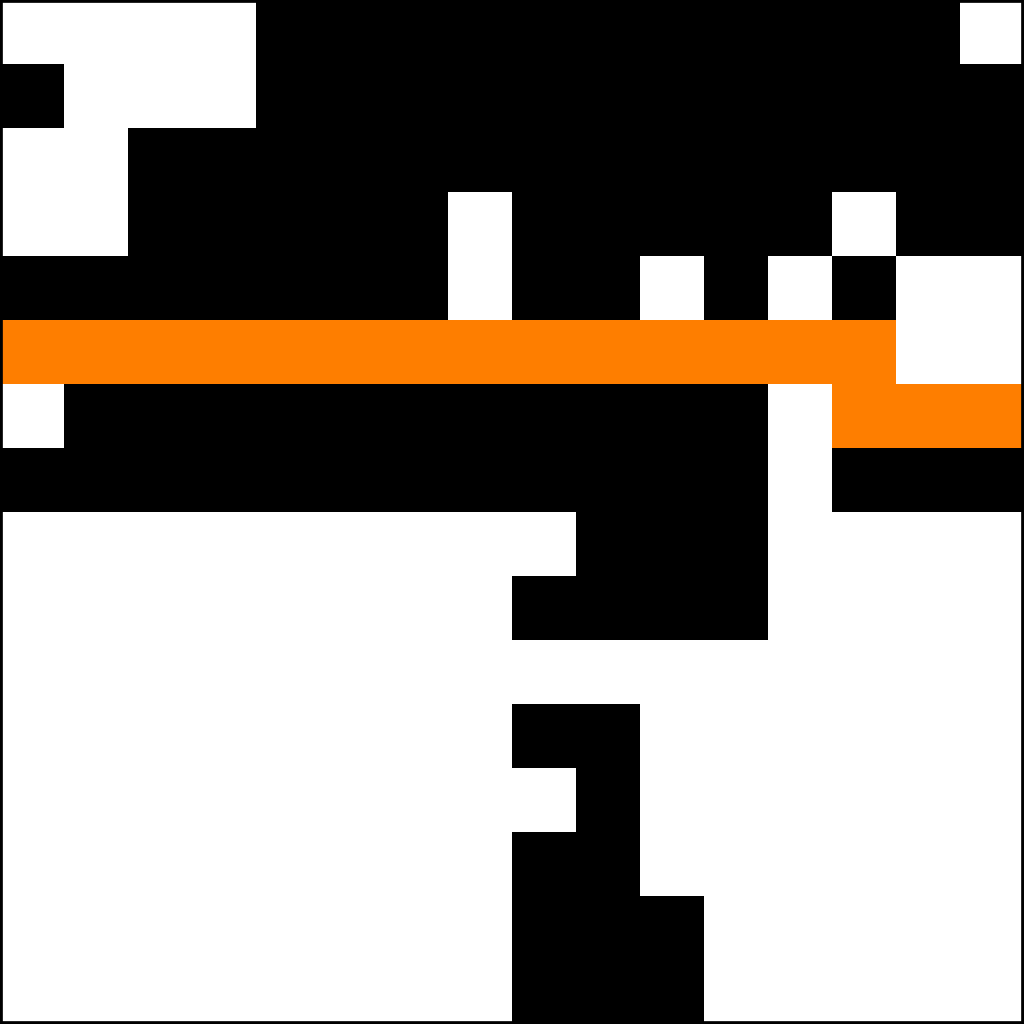
\includegraphics[scale=1.25]{imgs/perc2step4_crossing.png}}
			\only<11>{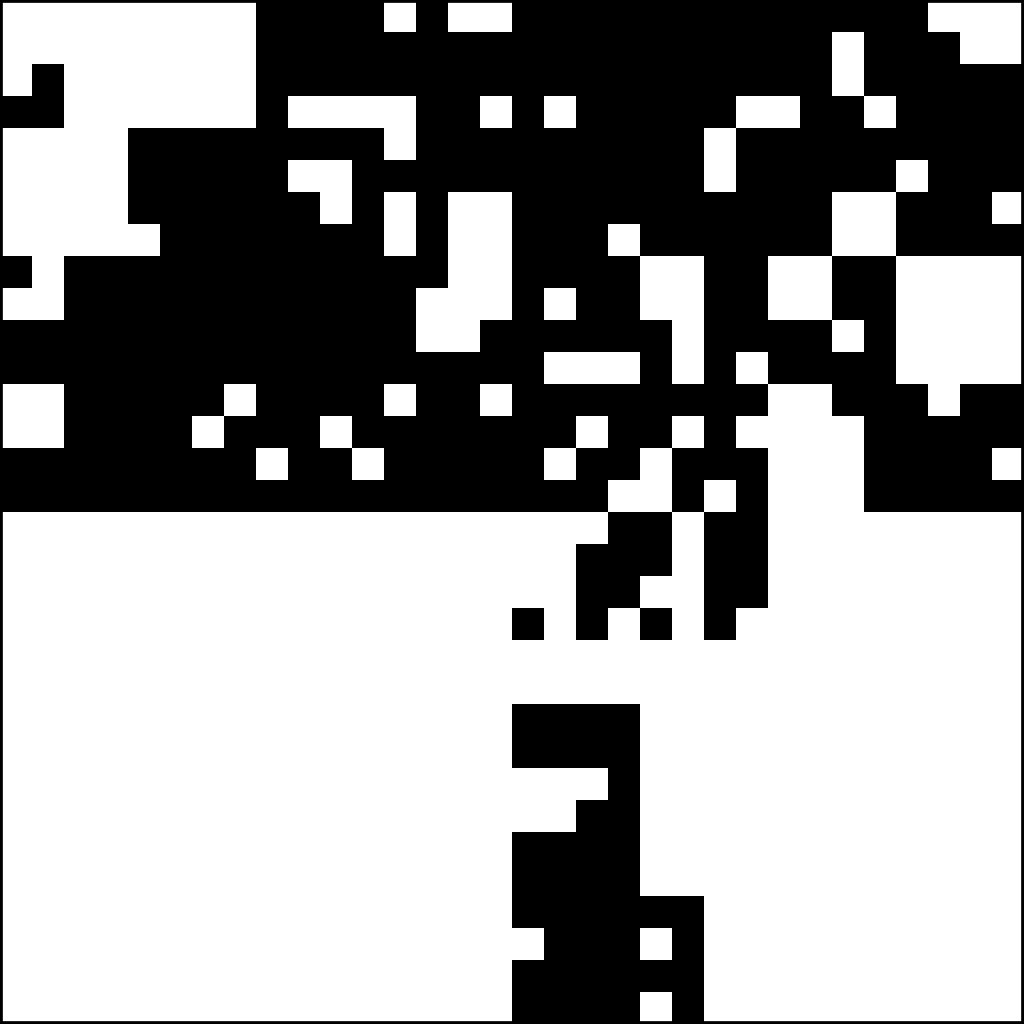
\includegraphics[scale=1.25]{imgs/perc2step5.png}}
			\only<12>{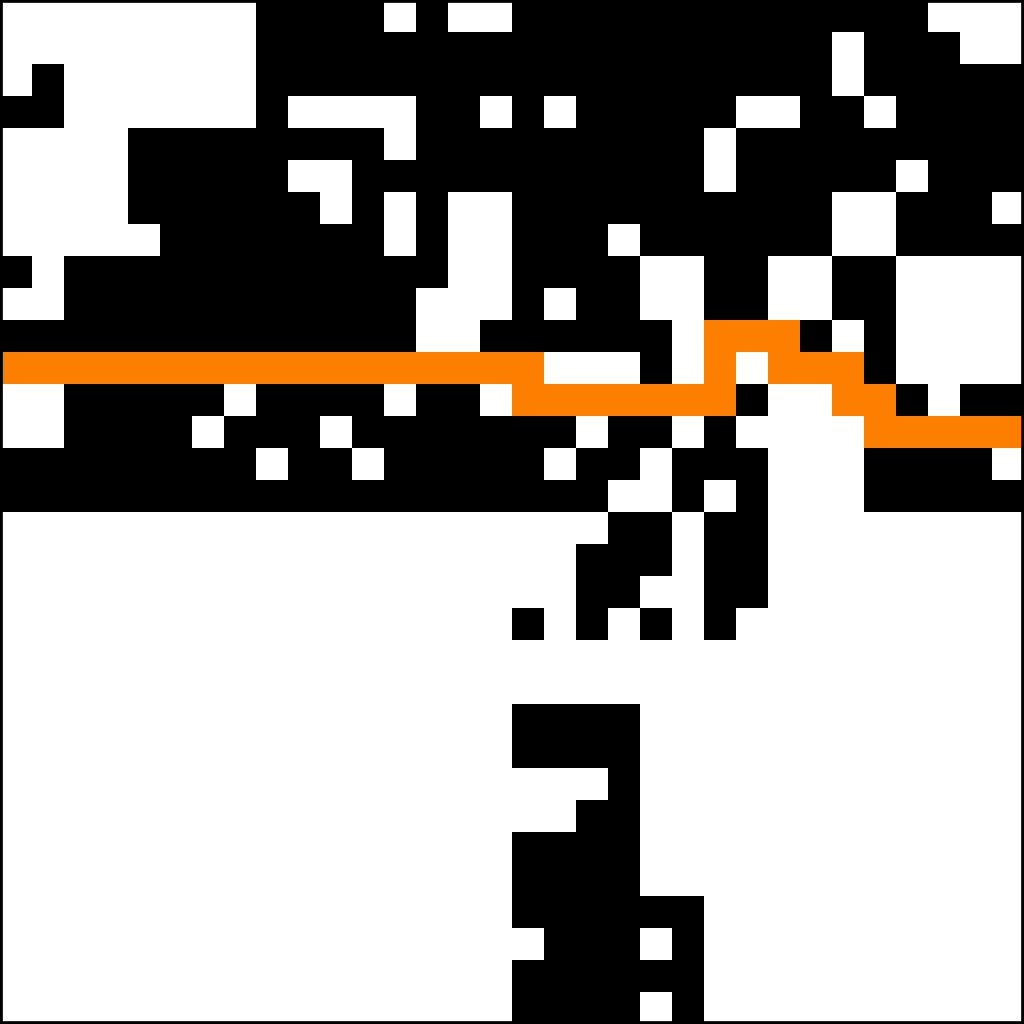
\includegraphics[scale=1.25]{imgs/perc2step5_crossing.png}}
			\only<13>{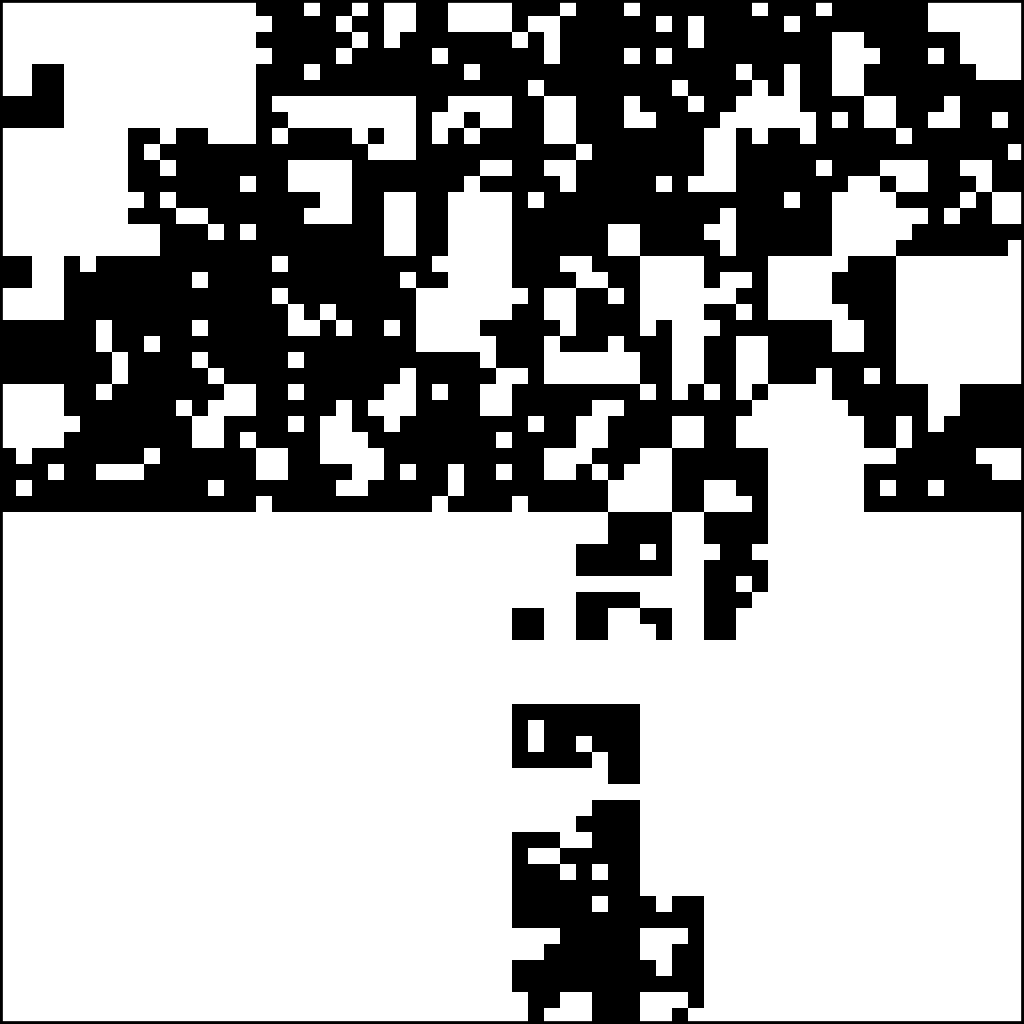
\includegraphics[scale=1.25]{imgs/perc2step6.png}}
			\only<14>{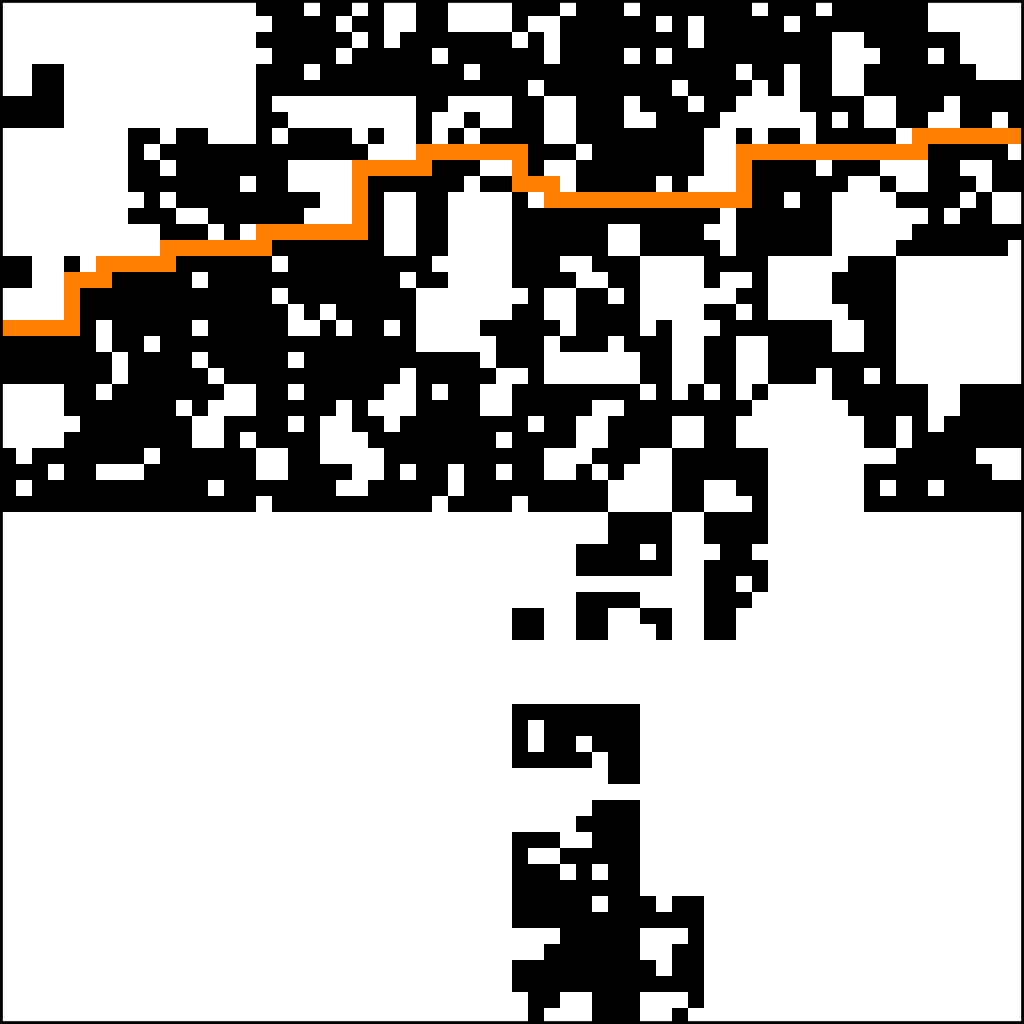
\includegraphics[scale=1.25]{imgs/perc2step6_crossing.png}}
			\only<15>{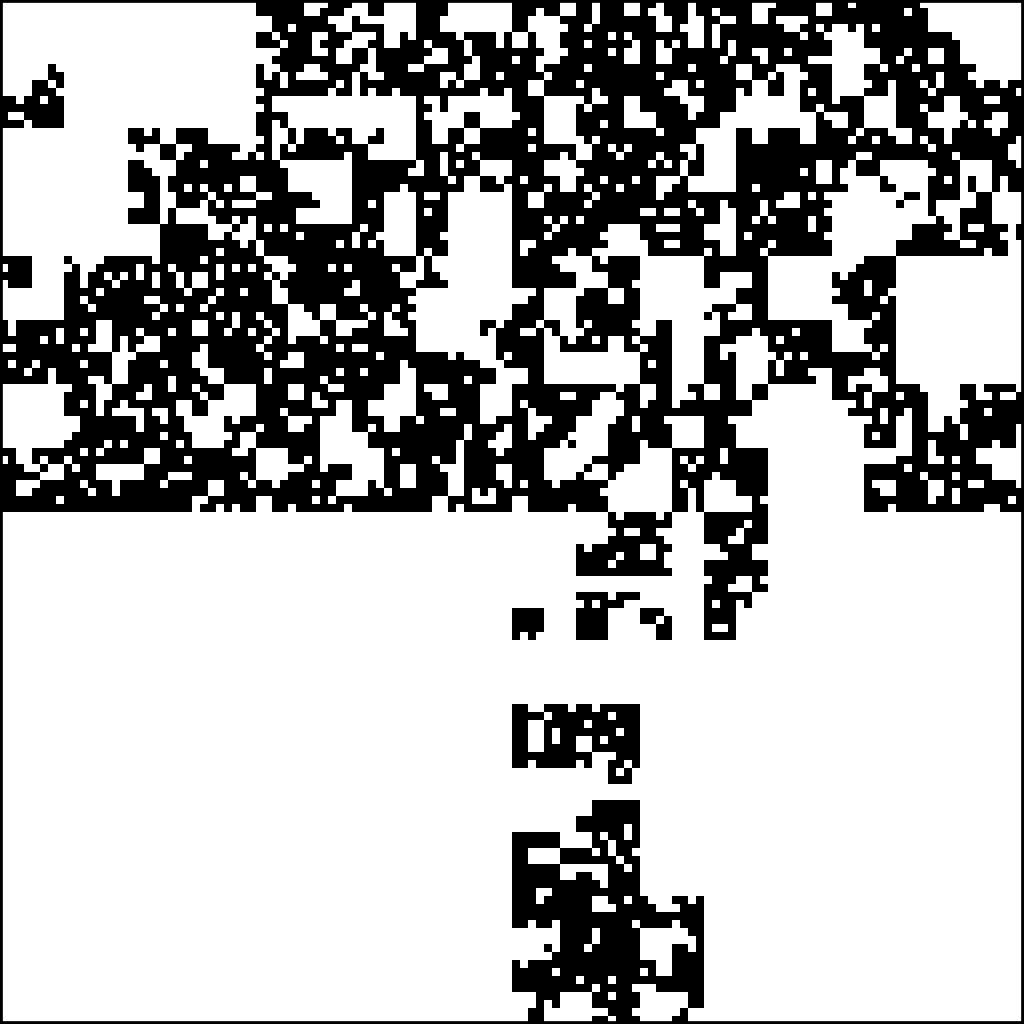
\includegraphics[scale=1.25]{imgs/perc2step7.png}}
			\only<16>{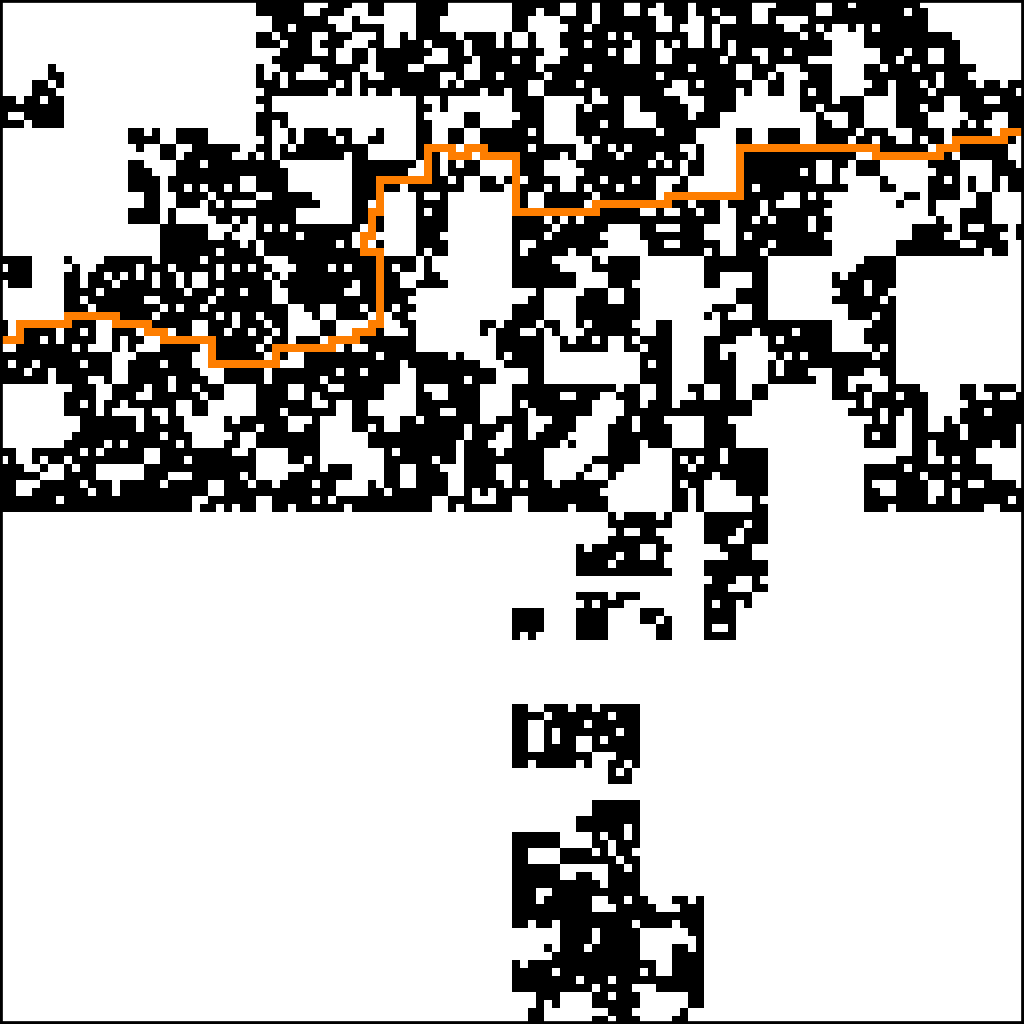
\includegraphics[scale=1.25]{imgs/perc2step7_crossing.png}}
			\only<17>{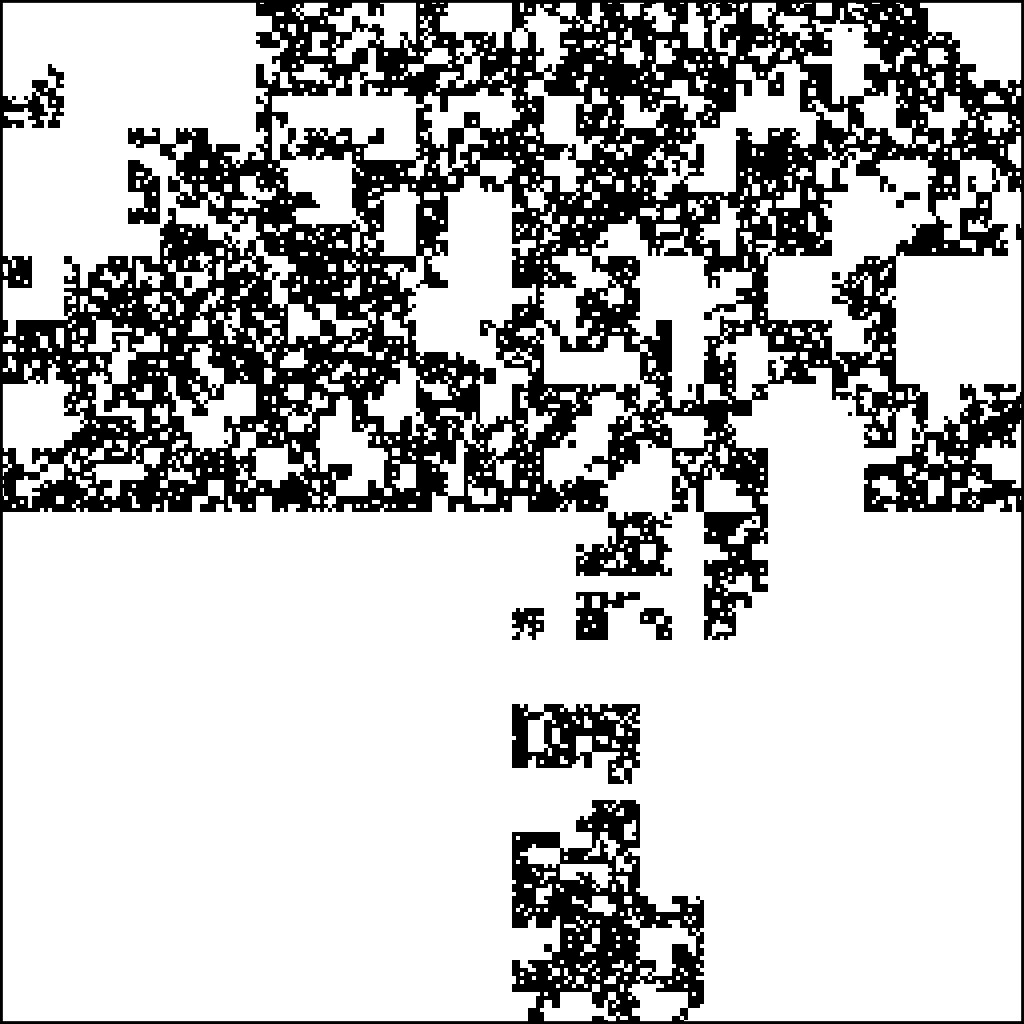
\includegraphics[scale=1.25]{imgs/perc2step8.png}}
			\only<18>{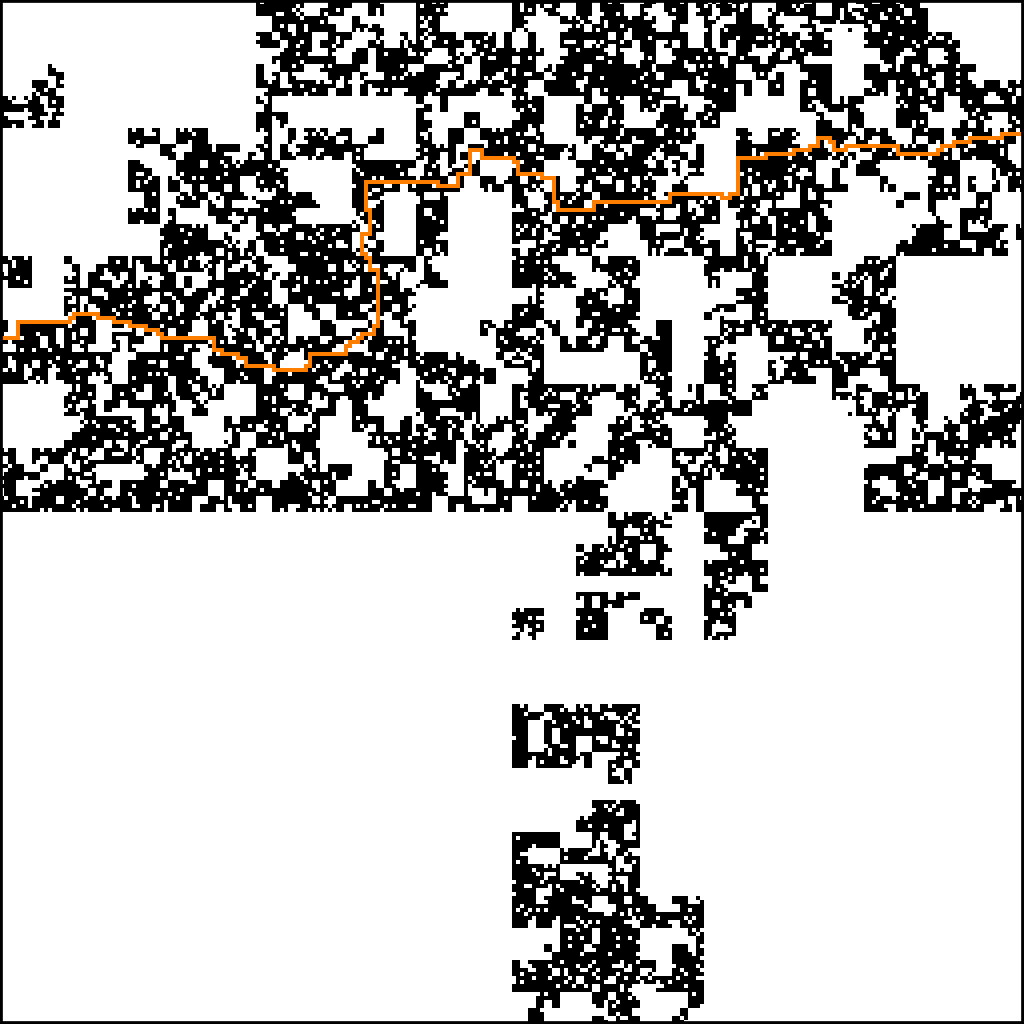
\includegraphics[scale=1.25]{imgs/perc2step8_crossing.png}}
			\only<19>{\includegraphics[scale=1.25]{imgs/perc2step9.png}}
			\only<20>{\includegraphics[scale=1.25]{imgs/perc2step9_crossing.png}}
		\end{center}
	\end{frame}
	\begin{frame}
		\frametitle{Finding Crossings}
		\framesubtitle{Example for $n=3$}
		\begin{center}
			\only<1>{\includegraphics[scale=0.85]{imgs/perc3step0.png}}
			\only<2>{\includegraphics[scale=0.85]{imgs/perc3step0_crossing.png}}
			\only<3>{\includegraphics[scale=0.85]{imgs/perc3step1.png}}
			\only<4>{\includegraphics[scale=0.85]{imgs/perc3step1_crossing.png}}
			\only<5>{\includegraphics[scale=0.85]{imgs/perc3step2.png}}
			\only<6>{\includegraphics[scale=0.85]{imgs/perc3step2_crossing.png}}
			\only<7>{\includegraphics[scale=0.85]{imgs/perc3step3.png}}
			\only<8>{\includegraphics[scale=0.85]{imgs/perc3step3_crossing.png}}
			\only<9>{\includegraphics[scale=0.85]{imgs/perc3step4.png}}
			\only<10>{\includegraphics[scale=0.85]{imgs/perc3step4_crossing.png}}
			\only<11>{\includegraphics[scale=0.85]{imgs/perc3step5.png}}
			\only<12>{\includegraphics[scale=0.85]{imgs/perc3step5_crossing.png}}
		\end{center}
	\end{frame}
	\begin{frame}
		\frametitle{Finding Crossings}
		\framesubtitle{Example for $n=5$}
		\begin{center}
			\only<1>{\includegraphics[scale=0.5]{imgs/perc5step0.png}}
			\only<2>{\includegraphics[scale=0.5]{imgs/perc5step0_crossing.png}}
			\only<3>{\includegraphics[scale=0.5]{imgs/perc5step1.png}}
			\only<4>{\includegraphics[scale=0.5]{imgs/perc5step1_crossing.png}}
			\only<5>{\includegraphics[scale=0.5]{imgs/perc5step2.png}}
			\only<6>{\includegraphics[scale=0.5]{imgs/perc5step2_crossing.png}}
			\only<7>{\includegraphics[scale=0.5]{imgs/perc5step3.png}}
			\only<8>{\includegraphics[scale=0.5]{imgs/perc5step3_crossing.png}}
		\end{center}
	\end{frame}

	\begin{frame}
		\frametitle{Crossings}
		\framesubtitle{straight}
		% 3 types
		% algo
		% results: straight, semi-straight, any
		% straight theory 
		% 
	\end{frame}
	
	
	\begin{frame}
	    \frametitle{Blob}
	    % data
		% random walks%
		%universe?
	\end{frame}
	

\end{document}
